% Generated by scripts/build_portrait_gallery.py; do not edit by hand.
% One page is emitted for each tagged person.
\begingroup
\definecolor{GalleryBordeaux}{HTML}{7C2F3A}
\definecolor{GalleryTerracotta}{HTML}{B55A52}
\definecolor{GalleryCream}{HTML}{F7F1ED}
\definecolor{GallerySand}{HTML}{DEC9C3}
\definecolor{GalleryInk}{HTML}{242321}
\definecolor{GalleryMuted}{HTML}{68655F}
\newcommand{\gallerypageheader}{%
  \begingroup\setlength{\fboxsep}{6pt}%
  \noindent\colorbox{GalleryBordeaux}{\parbox{\dimexpr\textwidth-2\fboxsep\relax}{%
    {\small\bfseries\color{white}\MakeUppercase{Galerie de portraits}}%
    \hfill{\footnotesize\color{white}Mémoires de Benoît Coste}}}\par%
  \endgroup\vspace{0.42cm}%
}
\newcommand{\galleryfact}[2]{%
  {\footnotesize\bfseries\color{GalleryBordeaux}\MakeUppercase{#1}}\par%
  {\small\color{GalleryInk}#2}\par\vspace{0.45em}%
}
\newcommand{\gallerysection}[1]{%
  {\footnotesize\bfseries\color{GalleryBordeaux}\MakeUppercase{#1}}\par%
}
\newcommand{\galleryworkline}[2]{%
  {\scriptsize\bfseries\color{GalleryBordeaux}#1 : }%
  {\scriptsize\color{GalleryInk}#2}\par%
}
\newcommand{\galleryworktitle}[1]{%
  {\scriptsize\bfseries\color{GalleryInk}#1}\par%
}
\clearpage
\thispagestyle{plain}
\begingroup
\newgeometry{top=1.15cm,bottom=1.25cm,left=1.30cm,right=1.30cm}
\raggedbottom
\phantomsection\addcontentsline{toc}{section}{Galerie de portraits}
\gallerypageheader
{\LARGE\bfseries\color{GalleryInk} Benoit COSTE}\par
\vspace{0.12cm}
\noindent\textcolor{GallerySand}{\rule{\textwidth}{1.1pt}}\par
\vspace{0.15cm}
{\footnotesize\bfseries\color{GalleryMuted}\MakeUppercase{Relation avec Benoît Coste}}\par
{\large\color{GalleryBordeaux} Lui-même}\par
\vspace{0.45cm}
\noindent\begin{minipage}[t]{0.52\textwidth}
\noindent\setlength{\fboxsep}{8pt}\colorbox{GalleryCream}{\parbox[t]{\dimexpr\linewidth-2\fboxsep\relax}{\galleryfact{Naissance}{7 avril 1781 — Lyon}
\galleryfact{Décès}{31 décembre 1845 — Montréal}}}
\end{minipage}\hfill
\begin{minipage}[t]{0.43\textwidth}\centering
\setlength{\fboxsep}{4pt}\setlength{\fboxrule}{0.8pt}\fcolorbox{GalleryTerracotta}{white}{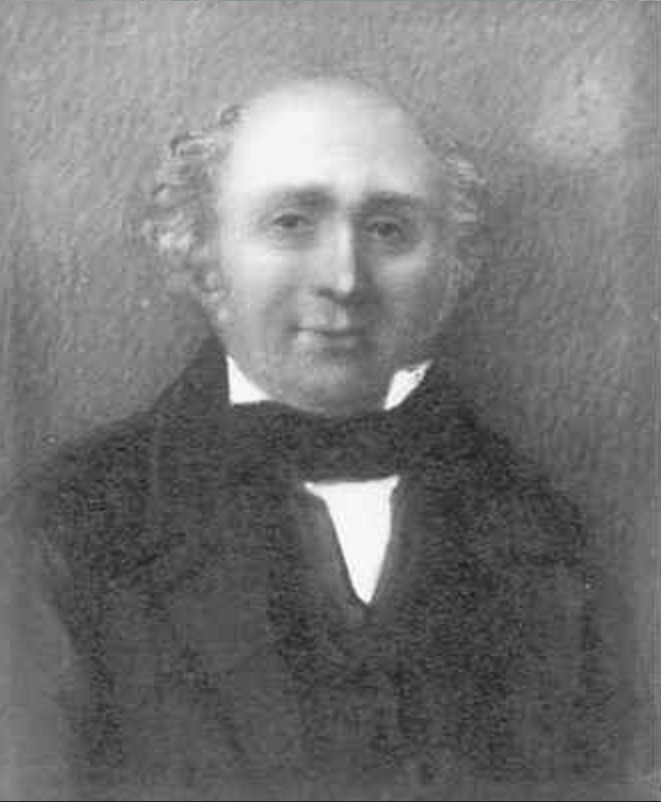
\includegraphics[width=0.88\linewidth,height=0.40\textheight,keepaspectratio]{genealogie/assets/galerie/portraits/portrait-15847fa5936f12e6c609.jpg}}
\par\vspace{0.10cm}
\galleryworktitle{Portrait de Benoit Coste}
\galleryworkline{Source}{\href{https://www.geneanet.org/media/public/benoit-coste-48840030}{Source en ligne}}
\end{minipage}
\vfill
\noindent\textcolor{GallerySand}{\rule{\textwidth}{0.6pt}}\par
{\scriptsize\color{GalleryMuted}Personnage cité dans les Mémoires de Benoît Coste}\par
\restoregeometry
\endgroup

\clearpage
\thispagestyle{plain}
\begingroup
\newgeometry{top=1.15cm,bottom=1.25cm,left=1.30cm,right=1.30cm}
\raggedbottom

\gallerypageheader
{\LARGE\bfseries\color{GalleryInk} Antoinette \underline{Joséphine} COLOMB DE GAST}\par
\vspace{0.12cm}
\noindent\textcolor{GallerySand}{\rule{\textwidth}{1.1pt}}\par
\vspace{0.15cm}
{\footnotesize\bfseries\color{GalleryMuted}\MakeUppercase{Relation avec Benoît Coste}}\par
{\large\color{GalleryBordeaux} Son épouse}\par
\vspace{0.45cm}
\noindent\begin{minipage}[t]{0.52\textwidth}
\noindent\setlength{\fboxsep}{8pt}\colorbox{GalleryCream}{\parbox[t]{\dimexpr\linewidth-2\fboxsep\relax}{\galleryfact{Naissance}{11 mai 1787 — Saint-Chamond}
\galleryfact{Décès}{12 mars 1855 — Saint-Étienne}
\galleryfact{Profession}{Non renseignée}}}
\end{minipage}\hfill
\begin{minipage}[t]{0.43\textwidth}\centering
\setlength{\fboxsep}{4pt}\setlength{\fboxrule}{0.8pt}\fcolorbox{GalleryTerracotta}{white}{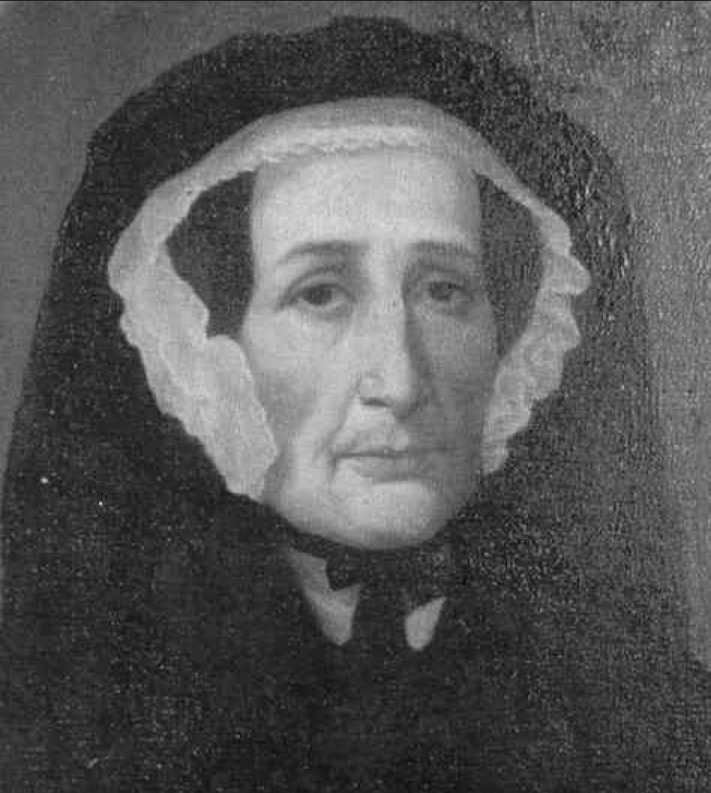
\includegraphics[width=0.88\linewidth,height=0.40\textheight,keepaspectratio]{genealogie/assets/galerie/portraits/portrait-5e1a47e248be410d4037.jpg}}
\par\vspace{0.10cm}
\galleryworktitle{Portrait de Antoinette Joséphine COLOMB DE GAST}
\galleryworkline{Source}{\href{https://www.geneanet.org/media/public/antoinette-josephine-colomb-de-gast-49545879}{Source en ligne}}
\end{minipage}
\par\vspace{0.30cm}
\noindent\setlength{\fboxsep}{6pt}\colorbox{GalleryCream}{
\parbox[t]{\dimexpr\linewidth-2\fboxsep-0.4cm\relax}{
\gallerysection{Citations dans l'ouvrage}
{\scriptsize\itshape\color{GalleryMuted} Benoît Coste — Mes souvenirs de soixante ans}\par\vspace{0.10cm}
{\footnotesize\begin{itemize}\setlength{\itemsep}{0pt}\setlength{\topsep}{1pt}\setlength{\parsep}{0pt}\setlength{\parskip}{0pt}
\item Chapitre 15 — p. 110 — \textit{« l’époque si heureuse de mon union avec votre excellente mère et la douce alliance contractée avec votre mère. »}
\item Chapitre 15 — p. 113 — \textit{« Mademoiselle Joséphine, puis ma future épouse, lors de la rencontre avec la famille Colomb. »}
\item Chapitre 15 — p. 114 — \textit{« le 14 Juillet 1807 Monsieur Ribière acheva son ouvrage en nous donnant la bénédiction nuptiale. »}
\item Chapitre 16 — p. 117 — \textit{« ma femme vivement affectée par le départ de Catherine, puis décrite comme ma bien aimée femme et une épouse attentive à ses devoirs. »}
\end{itemize}}
}
}
\vfill
\noindent\textcolor{GallerySand}{\rule{\textwidth}{0.6pt}}\par
{\scriptsize\color{GalleryMuted}Personnage cité dans les Mémoires de Benoît Coste}\par
\restoregeometry
\endgroup

\clearpage
\thispagestyle{plain}
\begingroup
\newgeometry{top=1.15cm,bottom=1.25cm,left=1.30cm,right=1.30cm}
\raggedbottom

\gallerypageheader
{\LARGE\bfseries\color{GalleryInk} \underline{François} Marie Isaac COSTE}\par
\vspace{0.12cm}
\noindent\textcolor{GallerySand}{\rule{\textwidth}{1.1pt}}\par
\vspace{0.15cm}
{\footnotesize\bfseries\color{GalleryMuted}\MakeUppercase{Relation avec Benoît Coste}}\par
{\large\color{GalleryBordeaux} Son fils}\par
\vspace{0.45cm}
\noindent\begin{minipage}[t]{0.52\textwidth}
\noindent\setlength{\fboxsep}{8pt}\colorbox{GalleryCream}{\parbox[t]{\dimexpr\linewidth-2\fboxsep\relax}{\galleryfact{Naissance}{9 novembre 1822}
\galleryfact{Décès}{Non renseignée}
\galleryfact{Profession}{Non renseignée}}}
\end{minipage}\hfill
\begin{minipage}[t]{0.43\textwidth}\centering
\setlength{\fboxsep}{4pt}\setlength{\fboxrule}{0.8pt}\fcolorbox{GalleryTerracotta}{white}{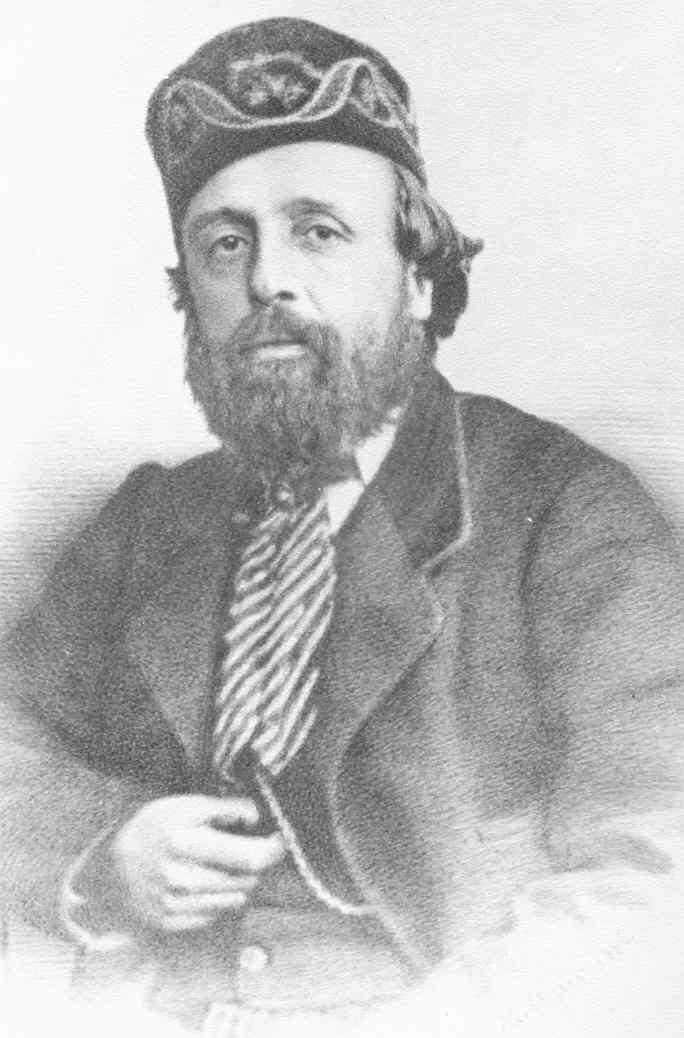
\includegraphics[width=0.88\linewidth,height=0.40\textheight,keepaspectratio]{genealogie/assets/galerie/portraits/portrait-81343f74c736103d4e28.jpg}}
\par\vspace{0.10cm}
\galleryworktitle{Portrait de François Coste}
\galleryworkline{Source}{\href{https://www.geneanet.org/media/public/1019238-jpg-2932143}{Source en ligne}}
\end{minipage}
\par\vspace{0.30cm}
\noindent\setlength{\fboxsep}{6pt}\colorbox{GalleryCream}{
\parbox[t]{\dimexpr\linewidth-2\fboxsep-0.4cm\relax}{
\gallerysection{Citations dans l'ouvrage}
{\scriptsize\itshape\color{GalleryMuted} Benoît Coste — Mes souvenirs de soixante ans}\par\vspace{0.10cm}
{\footnotesize\begin{itemize}\setlength{\itemsep}{0pt}\setlength{\topsep}{1pt}\setlength{\parsep}{0pt}\setlength{\parskip}{0pt}
\item Chapitre 26 — p. 212 — \textit{« Tu vins au monde le 9 du mois de novembre 1822... tu fus baptisé le jour même de ta naissance ; tu reçus sur les fonts du baptême, les noms de François, Marie Isaac »}
\item Chapitre 31 — p. 255 — \textit{« mon François qui étant aux Minimes, seul de mon petit troupeau, n’était pas alors dans mon bercail »}
\item Chapitre 33 — p. 266 — \textit{« tu fus admis... à la Table Sainte, vers le mois de mai 1833. Ce fut dans l’Église de St Polycarpe »}
\item Chapitre 33 — p. 267 — \textit{« Tu fus admis, un mois et demi environ après ta première Communion, à recevoir le Sacrement de Confirmation »}
\item Chapitre 33 — p. 267 — \textit{« Tu y fis ton entrée vers le milieu d’octobre 1833 »}
\end{itemize}}
}
}
\vfill
\noindent\textcolor{GallerySand}{\rule{\textwidth}{0.6pt}}\par
{\scriptsize\color{GalleryMuted}Personnage cité dans les Mémoires de Benoît Coste}\par
\restoregeometry
\endgroup

\clearpage
\thispagestyle{plain}
\begingroup
\newgeometry{top=1.15cm,bottom=1.25cm,left=1.30cm,right=1.30cm}
\raggedbottom

\gallerypageheader
{\LARGE\bfseries\color{GalleryInk} Isaac COSTE}\par
\vspace{0.12cm}
\noindent\textcolor{GallerySand}{\rule{\textwidth}{1.1pt}}\par
\vspace{0.15cm}
{\footnotesize\bfseries\color{GalleryMuted}\MakeUppercase{Relation avec Benoît Coste}}\par
{\large\color{GalleryBordeaux} Son père}\par
\vspace{0.45cm}
\noindent\begin{minipage}[t]{0.52\textwidth}
\noindent\setlength{\fboxsep}{8pt}\colorbox{GalleryCream}{\parbox[t]{\dimexpr\linewidth-2\fboxsep\relax}{\galleryfact{Naissance}{Non renseignée}
\galleryfact{Décès}{27 octobre 1802 — Lyon}
\gallerysection{Profession}
\small\begin{itemize}\setlength{\itemsep}{0pt}\setlength{\topsep}{2pt}\setlength{\parsep}{0pt}\setlength{\parskip}{0pt}
\item Échevin
\item Marchand de soie.
\item Agent de change . A transmis cette charge à Benoît Coste en 1803.
\end{itemize}}}
\end{minipage}\hfill
\begin{minipage}[t]{0.43\textwidth}\centering
\setlength{\fboxsep}{4pt}\setlength{\fboxrule}{0.8pt}\fcolorbox{GalleryTerracotta}{white}{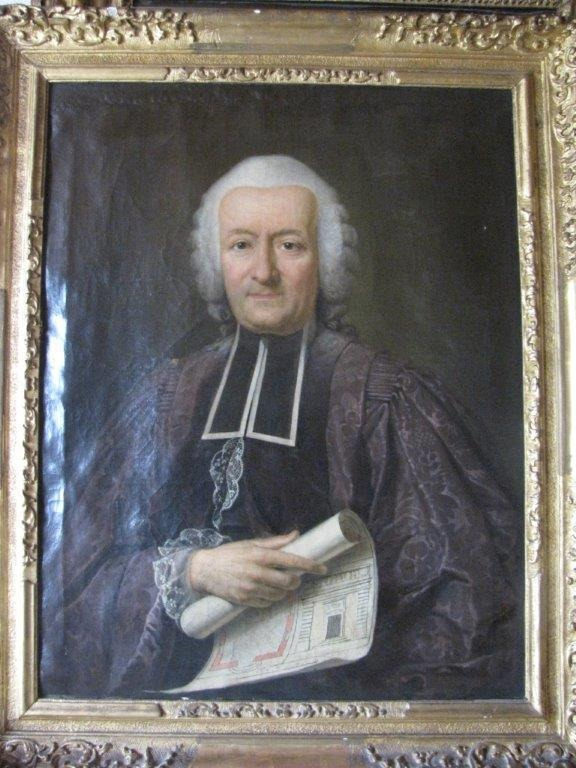
\includegraphics[width=0.88\linewidth,height=0.40\textheight,keepaspectratio]{genealogie/assets/galerie/portraits/portrait-44af026de86cb794bcf2.jpg}}
\par\vspace{0.10cm}
\galleryworktitle{Portrait d’Isaac Coste en tenue d’échevin}
\galleryworkline{Source}{\href{https://www.geneanet.org/media/public/64-reduite-15791938}{Source en ligne}}
\end{minipage}
\par\vspace{0.30cm}
\noindent\setlength{\fboxsep}{6pt}\colorbox{GalleryCream}{
\parbox[t]{\dimexpr\linewidth-2\fboxsep-0.4cm\relax}{
\gallerysection{Citations dans l'ouvrage}
{\scriptsize\itshape\color{GalleryMuted} Benoît Coste — Mes souvenirs de soixante ans}\par\vspace{0.10cm}
{\footnotesize\begin{itemize}\setlength{\itemsep}{0pt}\setlength{\topsep}{1pt}\setlength{\parsep}{0pt}\setlength{\parskip}{0pt}
\item Chapitre 1 — p. 6 — \textit{« Mon père était marchand de soie »}
\item Chapitre 2 — p. 16 — \textit{« Mon père fut averti et eut le bonheur d'être du petit nombre de ceux qui parvinrent à s'échapper. J'étais instruit de sa condamnation, je savais que, le jour même (jour mémorable, c'était le 11 décembre), il devait être exécuté »}
\item Chapitre 2 — p. 17 — \textit{« Vers la fin du mois de décembre, à l'aide de faux papiers, il parvint à gagner la Suisse. »}
\item Chapitre 4 — p. 25 — \textit{« Mon père nous avait quittés vers la fin de 1795, ou au printemps de 1796. »}
\item Chapitre 9 — p. 65 — \textit{« La compagnie des agents de change avait été rétablie à Lyon en 1801... Il prit donc le parti... de se mettre lui-même sur les rangs... Il n'exerça que quelques mois »}
\item Chapitre 11 — p. 82 — \textit{« Le 27 octobre 1802 à neuf heures du soir, je passai une demi-heure auprès de son lit... à onze heures du soir... un vomissement de sang venait de l'enlever en quelques secondes. »}
\item Chapitre 11 — p. 82 — \textit{« Les obsèques de mon père eurent lieu dans l'oratoire de St Irénée... le convoi... s'achemina jusqu'au cimetière dit de St Just, près du télégraphe. »}
\end{itemize}}
}
}
\vfill
\noindent\textcolor{GallerySand}{\rule{\textwidth}{0.6pt}}\par
{\scriptsize\color{GalleryMuted}Personnage cité dans les Mémoires de Benoît Coste}\par
\restoregeometry
\endgroup

\clearpage
\thispagestyle{plain}
\begingroup
\newgeometry{top=1.15cm,bottom=1.25cm,left=1.30cm,right=1.30cm}
\raggedbottom

\gallerypageheader
{\LARGE\bfseries\color{GalleryInk} Jeanne Françoise \underline{Marie} COSTE}\par
\vspace{0.12cm}
\noindent\textcolor{GallerySand}{\rule{\textwidth}{1.1pt}}\par
\vspace{0.15cm}
{\footnotesize\bfseries\color{GalleryMuted}\MakeUppercase{Relation avec Benoît Coste}}\par
{\large\color{GalleryBordeaux} Sa fille}\par
\vspace{0.45cm}
\noindent\begin{minipage}[t]{0.52\textwidth}
\noindent\setlength{\fboxsep}{8pt}\colorbox{GalleryCream}{\parbox[t]{\dimexpr\linewidth-2\fboxsep\relax}{\galleryfact{Naissance}{23 juillet 1818 — Lyon}
\galleryfact{Décès}{1 décembre 1862 — 10 montée des Carmes Déchaussées, Lyon 5e}
\gallerysection{Profession}
\small\begin{itemize}\setlength{\itemsep}{0pt}\setlength{\topsep}{2pt}\setlength{\parsep}{0pt}\setlength{\parskip}{0pt}
\item Sans profession (acte de décès de Jeanne Françoise Marie Coste)
\end{itemize}}}
\end{minipage}\hfill
\begin{minipage}[t]{0.43\textwidth}\centering
\setlength{\fboxsep}{4pt}\setlength{\fboxrule}{0.8pt}\fcolorbox{GalleryTerracotta}{white}{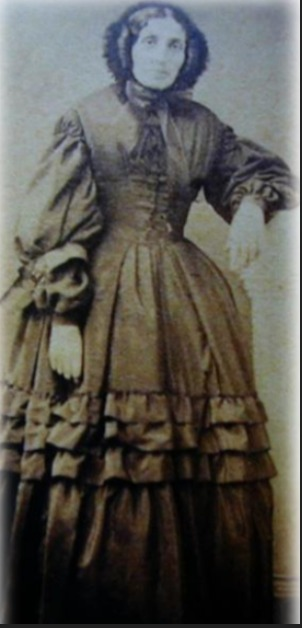
\includegraphics[width=0.88\linewidth,height=0.40\textheight,keepaspectratio]{genealogie/assets/galerie/portraits/portrait-bdc81249726a0bb26360.jpg}}
\par\vspace{0.10cm}
\galleryworktitle{Photo de Jeanne Coste}
\galleryworkline{Source}{\href{https://www.geneanet.org/media/public/photo-coste-jeanne-2-francoise-marie-15180206}{Source en ligne}}
\end{minipage}
\par\vspace{0.30cm}
\noindent\setlength{\fboxsep}{6pt}\colorbox{GalleryCream}{
\parbox[t]{\dimexpr\linewidth-2\fboxsep-0.4cm\relax}{
\gallerysection{Citations dans l'ouvrage}
{\scriptsize\itshape\color{GalleryMuted} Benoît Coste — Mes souvenirs de soixante ans}\par\vspace{0.10cm}
{\footnotesize\begin{itemize}\setlength{\itemsep}{0pt}\setlength{\topsep}{1pt}\setlength{\parsep}{0pt}\setlength{\parskip}{0pt}
\item Chapitre 24 — p. 192 — \textit{« Tu vins au monde le 23 juillet 1818, tu fus baptisée le lendemain ; on te donna sur les fonts du baptême les noms de Jeanne Françoise Marie »}
\item Chapitre 33 — p. 265 — \textit{« Votre séjour dans le pensionnat de Brignais avait été de cinq ans. »}
\item Chapitre 33 — p. 270 — \textit{« Monsieur Guérin, notre excellent oncle... voulut bien être son parrain ; Marie fut sa marraine. »}
\end{itemize}}
}
}
\vfill
\noindent\textcolor{GallerySand}{\rule{\textwidth}{0.6pt}}\par
{\scriptsize\color{GalleryMuted}Personnage cité dans les Mémoires de Benoît Coste}\par
\restoregeometry
\endgroup

\clearpage
\thispagestyle{plain}
\begingroup
\newgeometry{top=1.15cm,bottom=1.25cm,left=1.30cm,right=1.30cm}
\raggedbottom

\gallerypageheader
{\LARGE\bfseries\color{GalleryInk} Marie Antoinette \underline{Blandine} COSTE}\par
\vspace{0.12cm}
\noindent\textcolor{GallerySand}{\rule{\textwidth}{1.1pt}}\par
\vspace{0.15cm}
{\footnotesize\bfseries\color{GalleryMuted}\MakeUppercase{Relation avec Benoît Coste}}\par
{\large\color{GalleryBordeaux} Sa fille}\par
\vspace{0.45cm}
\noindent\begin{minipage}[t]{0.52\textwidth}
\noindent\setlength{\fboxsep}{8pt}\colorbox{GalleryCream}{\parbox[t]{\dimexpr\linewidth-2\fboxsep\relax}{\galleryfact{Naissance}{13 avril 1820}
\galleryfact{Décès}{1890}
\gallerysection{Profession}
\small\begin{itemize}\setlength{\itemsep}{0pt}\setlength{\topsep}{2pt}\setlength{\parsep}{0pt}\setlength{\parskip}{0pt}
\item Religieuse du Sacré-Coeur
\end{itemize}}}
\end{minipage}\hfill
\begin{minipage}[t]{0.43\textwidth}\centering
\setlength{\fboxsep}{0pt}\setlength{\fboxrule}{0.8pt}
\fcolorbox{GallerySand}{GalleryCream}{
\parbox[c][0.50\textheight][c]{0.90\linewidth}{\centering
{\fontsize{48}{54}\selectfont\bfseries\color{GalleryBordeaux} BC}\par\medskip
{\small\color{GalleryMuted}Portrait non disponible}\par}}
\end{minipage}
\par\vspace{0.30cm}
\noindent\setlength{\fboxsep}{6pt}\colorbox{GalleryCream}{
\parbox[t]{\dimexpr\linewidth-2\fboxsep-0.4cm\relax}{
\gallerysection{Citations dans l'ouvrage}
{\scriptsize\itshape\color{GalleryMuted} Benoît Coste — Mes souvenirs de soixante ans}\par\vspace{0.10cm}
{\footnotesize\begin{itemize}\setlength{\itemsep}{0pt}\setlength{\topsep}{1pt}\setlength{\parsep}{0pt}\setlength{\parskip}{0pt}
\item Chapitre 24 — p. 194 — \textit{« Tu vins au monde, le 13 avril 1820, tu fus baptisée le lendemain... tu reçus les noms de Marie Antoinette Blandine »}
\item Chapitre 33 — p. 265 — \textit{« Votre séjour dans le pensionnat de Brignais avait été de cinq ans. »}
\end{itemize}}
}
}
\vfill
\noindent\textcolor{GallerySand}{\rule{\textwidth}{0.6pt}}\par
{\scriptsize\color{GalleryMuted}Personnage cité dans les Mémoires de Benoît Coste}\par
\restoregeometry
\endgroup

\clearpage
\thispagestyle{plain}
\begingroup
\newgeometry{top=1.15cm,bottom=1.25cm,left=1.30cm,right=1.30cm}
\raggedbottom

\gallerypageheader
{\LARGE\bfseries\color{GalleryInk} Marie Louise Joséphine COSTE}\par
\vspace{0.12cm}
\noindent\textcolor{GallerySand}{\rule{\textwidth}{1.1pt}}\par
\vspace{0.15cm}
{\footnotesize\bfseries\color{GalleryMuted}\MakeUppercase{Relation avec Benoît Coste}}\par
{\large\color{GalleryBordeaux} Sa fille}\par
\vspace{0.45cm}
\noindent\begin{minipage}[t]{0.52\textwidth}
\noindent\setlength{\fboxsep}{8pt}\colorbox{GalleryCream}{\parbox[t]{\dimexpr\linewidth-2\fboxsep\relax}{\galleryfact{Naissance}{19 janvier 1834 — Lyon}
\galleryfact{Décès}{juin 1834}
\galleryfact{Profession}{Non renseignée}}}
\end{minipage}\hfill
\begin{minipage}[t]{0.43\textwidth}\centering
\setlength{\fboxsep}{0pt}\setlength{\fboxrule}{0.8pt}
\fcolorbox{GallerySand}{GalleryCream}{
\parbox[c][0.50\textheight][c]{0.90\linewidth}{\centering
{\fontsize{48}{54}\selectfont\bfseries\color{GalleryBordeaux} MC}\par\medskip
{\small\color{GalleryMuted}Portrait non disponible}\par}}
\end{minipage}
\par\vspace{0.30cm}
\noindent\setlength{\fboxsep}{6pt}\colorbox{GalleryCream}{
\parbox[t]{\dimexpr\linewidth-2\fboxsep-0.4cm\relax}{
\gallerysection{Citations dans l'ouvrage}
{\scriptsize\itshape\color{GalleryMuted} Benoît Coste — Mes souvenirs de soixante ans}\par\vspace{0.10cm}
{\footnotesize\begin{itemize}\setlength{\itemsep}{0pt}\setlength{\topsep}{1pt}\setlength{\parsep}{0pt}\setlength{\parskip}{0pt}
\item Chapitre 33 — p. 270 — \textit{« au mois de janvier 1834, une petite fille nous fut montrée... Nous l’appelâmes Marie Louise Joséphine »}
\item Chapitre 33 — p. 270 — \textit{« Monsieur Guérin, notre excellent oncle... voulut bien être son parrain ; Marie fut sa marraine. »}
\item Chapitre 33 — p. 270 — \textit{« elle n’avait pas encore six mois ; lorsqu’elle fut attaquée d’une inflammation d’entrailles... elle termina en ce monde, la courte existence de ma pauvre petite. »}
\end{itemize}}
}
}
\vfill
\noindent\textcolor{GallerySand}{\rule{\textwidth}{0.6pt}}\par
{\scriptsize\color{GalleryMuted}Personnage cité dans les Mémoires de Benoît Coste}\par
\restoregeometry
\endgroup

\clearpage
\thispagestyle{plain}
\begingroup
\newgeometry{top=1.15cm,bottom=1.25cm,left=1.30cm,right=1.30cm}
\raggedbottom

\gallerypageheader
{\LARGE\bfseries\color{GalleryInk} \underline{Pierre} Marie Joseph COSTE}\par
\vspace{0.12cm}
\noindent\textcolor{GallerySand}{\rule{\textwidth}{1.1pt}}\par
\vspace{0.15cm}
{\footnotesize\bfseries\color{GalleryMuted}\MakeUppercase{Relation avec Benoît Coste}}\par
{\large\color{GalleryBordeaux} Son fils}\par
\vspace{0.45cm}
\noindent\begin{minipage}[t]{0.52\textwidth}
\noindent\setlength{\fboxsep}{8pt}\colorbox{GalleryCream}{\parbox[t]{\dimexpr\linewidth-2\fboxsep\relax}{\galleryfact{Naissance}{1824}
\galleryfact{Décès}{4 décembre 1828}
\galleryfact{Profession}{Non renseignée}}}
\end{minipage}\hfill
\begin{minipage}[t]{0.43\textwidth}\centering
\setlength{\fboxsep}{0pt}\setlength{\fboxrule}{0.8pt}
\fcolorbox{GallerySand}{GalleryCream}{
\parbox[c][0.50\textheight][c]{0.90\linewidth}{\centering
{\fontsize{48}{54}\selectfont\bfseries\color{GalleryBordeaux} PC}\par\medskip
{\small\color{GalleryMuted}Portrait non disponible}\par}}
\end{minipage}
\par\vspace{0.30cm}
\noindent\setlength{\fboxsep}{6pt}\colorbox{GalleryCream}{
\parbox[t]{\dimexpr\linewidth-2\fboxsep-0.4cm\relax}{
\gallerysection{Citations dans l'ouvrage}
{\scriptsize\itshape\color{GalleryMuted} Benoît Coste — Mes souvenirs de soixante ans}\par\vspace{0.10cm}
{\footnotesize\begin{itemize}\setlength{\itemsep}{0pt}\setlength{\topsep}{1pt}\setlength{\parsep}{0pt}\setlength{\parskip}{0pt}
\item Chapitre 26 — p. 217 — \textit{« 1824 – Naissance de Pierre... un quatrième enfant ; c’était encore un garçon ; nous l’appelâmes Pierre Marie Joseph, deux heures après sa naissance il eut le bonheur de recevoir le baptême. »}
\item Chapitre 28 — p. 231 — \textit{« le pauvre enfant fut bientôt après attaqué d’un tétanos... notre Pierre expira doucement dans nos bras le quatre décembre 1828 »}
\end{itemize}}
}
}
\vfill
\noindent\textcolor{GallerySand}{\rule{\textwidth}{0.6pt}}\par
{\scriptsize\color{GalleryMuted}Personnage cité dans les Mémoires de Benoît Coste}\par
\restoregeometry
\endgroup

\clearpage
\thispagestyle{plain}
\begingroup
\newgeometry{top=1.15cm,bottom=1.25cm,left=1.30cm,right=1.30cm}
\raggedbottom

\gallerypageheader
{\LARGE\bfseries\color{GalleryInk} Jeanne JORDAN}\par
\vspace{0.12cm}
\noindent\textcolor{GallerySand}{\rule{\textwidth}{1.1pt}}\par
\vspace{0.15cm}
{\footnotesize\bfseries\color{GalleryMuted}\MakeUppercase{Relation avec Benoît Coste}}\par
{\large\color{GalleryBordeaux} Sa mère}\par
\vspace{0.45cm}
\noindent\setlength{\fboxsep}{8pt}\colorbox{GalleryCream}{\parbox[t]{\dimexpr\linewidth-2\fboxsep\relax}{\galleryfact{Naissance}{1756}
\galleryfact{Décès}{13 octobre 1823 — Lyon}
\galleryfact{Profession}{Non renseignée}}}
\par\vspace{0.40cm}
\begin{minipage}[t]{0.475\linewidth}\centering
\setlength{\fboxsep}{4pt}\setlength{\fboxrule}{0.8pt}\fcolorbox{GalleryTerracotta}{white}{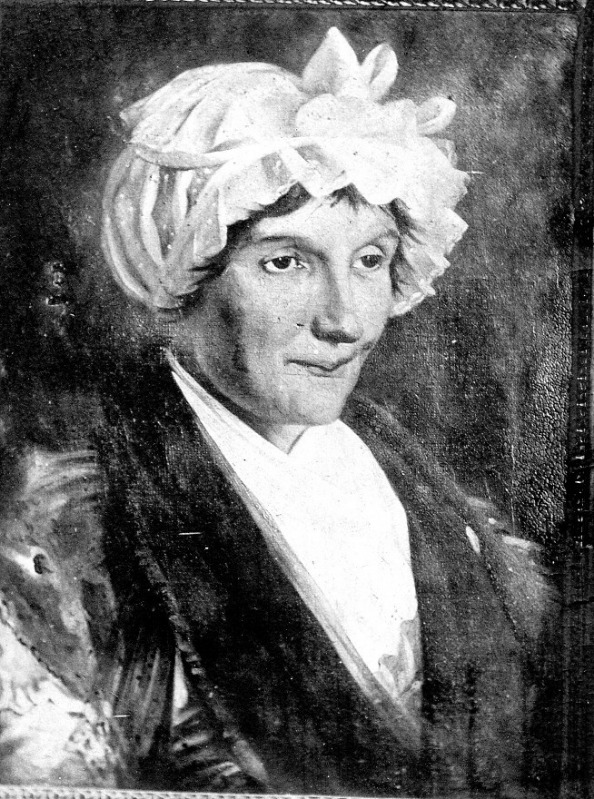
\includegraphics[width=0.88\linewidth,height=0.19\textheight,keepaspectratio]{genealogie/assets/galerie/portraits/portrait-06fbf8c6a24b9588094d.jpg}}
\par\vspace{0.10cm}
\galleryworktitle{Portrait de Jeanne JORDAN}
\galleryworkline{Source}{\href{https://www.geneanet.org/media/public/jeanne-jordan-48840009}{Source en ligne}}
\end{minipage}\hfill\begin{minipage}[t]{0.475\linewidth}\centering
\setlength{\fboxsep}{4pt}\setlength{\fboxrule}{0.8pt}\fcolorbox{GalleryTerracotta}{white}{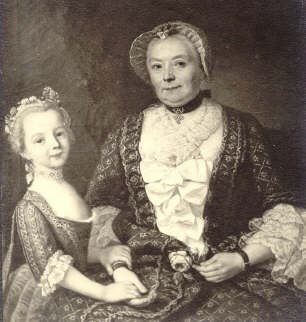
\includegraphics[width=0.88\linewidth,height=0.19\textheight,keepaspectratio]{genealogie/assets/galerie/portraits/portrait-7777f44e1b96ec0470ed.jpg}}
\par\vspace{0.10cm}
\galleryworktitle{Double portrait de Jeanne de Gérando et Jeanne Jordan}
\galleryworkline{Date}{1762}
\galleryworkline{Artiste}{Nonnotte Donat}
\galleryworkline{Source}{\href{https://www.geneanet.org/media/public/869698-jpg-2457452}{https://www.persee.fr/doc/bmml\_0521-7032\_1992\_num\_1992\_3\_1677 — p. 44, réf. 66}}
\end{minipage}
\par\vspace{0.30cm}
\noindent\setlength{\fboxsep}{6pt}\colorbox{GalleryCream}{
\parbox[t]{\dimexpr\linewidth-2\fboxsep-0.4cm\relax}{
\gallerysection{Citations dans l'ouvrage}
{\scriptsize\itshape\color{GalleryMuted} Benoît Coste — Mes souvenirs de soixante ans}\par\vspace{0.10cm}
{\footnotesize\begin{itemize}\setlength{\itemsep}{0pt}\setlength{\topsep}{1pt}\setlength{\parsep}{0pt}\setlength{\parskip}{0pt}
\item Chapitre 1 — p. 6 — \textit{« Ma mère, aussi fille d'un marchand de soie »}
\item Chapitre 11 — p. 83 — \textit{« pendant les 21 ans qu'elle lui a survécu »}
\item Chapitre 26 — p. 215 — \textit{« ma bonne et vertueuse mère rendit son âme à Dieu le dimanche 12 Octobre 1823, à neuf heures du matin »}
\end{itemize}}
}
}
\vfill
\noindent\textcolor{GallerySand}{\rule{\textwidth}{0.6pt}}\par
{\scriptsize\color{GalleryMuted}Personnage cité dans les Mémoires de Benoît Coste}\par
\restoregeometry
\endgroup

\clearpage
\thispagestyle{plain}
\begingroup
\newgeometry{top=1.15cm,bottom=1.25cm,left=1.30cm,right=1.30cm}
\raggedbottom

\gallerypageheader
{\LARGE\bfseries\color{GalleryInk} Claudine Marie \underline{Joséphine} BERLOTY}\par
\vspace{0.12cm}
\noindent\textcolor{GallerySand}{\rule{\textwidth}{1.1pt}}\par
\vspace{0.15cm}
{\footnotesize\bfseries\color{GalleryMuted}\MakeUppercase{Relation avec Benoît Coste}}\par
{\large\color{GalleryBordeaux} Sa petite-fille}\par
\vspace{0.45cm}
\noindent\begin{minipage}[t]{0.52\textwidth}
\noindent\setlength{\fboxsep}{8pt}\colorbox{GalleryCream}{\parbox[t]{\dimexpr\linewidth-2\fboxsep\relax}{\galleryfact{Naissance}{16 mars 1841 — Lyon}
\galleryfact{Décès}{30 janvier 1916 — 2 place de la Bourse, Lyon 2e}
\gallerysection{Profession}
\small\begin{itemize}\setlength{\itemsep}{0pt}\setlength{\topsep}{2pt}\setlength{\parsep}{0pt}\setlength{\parskip}{0pt}
\item Sans profession
\end{itemize}}}
\end{minipage}\hfill
\begin{minipage}[t]{0.43\textwidth}\centering
\setlength{\fboxsep}{0pt}\setlength{\fboxrule}{0.8pt}
\fcolorbox{GallerySand}{GalleryCream}{
\parbox[c][0.50\textheight][c]{0.90\linewidth}{\centering
{\fontsize{48}{54}\selectfont\bfseries\color{GalleryBordeaux} JB}\par\medskip
{\small\color{GalleryMuted}Portrait non disponible}\par}}
\end{minipage}
\par\vspace{0.30cm}
\noindent\setlength{\fboxsep}{6pt}\colorbox{GalleryCream}{
\parbox[t]{\dimexpr\linewidth-2\fboxsep-0.4cm\relax}{
\gallerysection{Citations dans l'ouvrage}
{\scriptsize\itshape\color{GalleryMuted} Benoît Coste — Mes souvenirs de soixante ans}\par\vspace{0.10cm}
{\footnotesize\begin{itemize}\setlength{\itemsep}{0pt}\setlength{\topsep}{1pt}\setlength{\parsep}{0pt}\setlength{\parskip}{0pt}
\item Chapitre 35 — p. 285 — \textit{« Naissance de ma première petite-fille... c’est à cette chère petite Joséphine »}
\end{itemize}}
}
}
\vfill
\noindent\textcolor{GallerySand}{\rule{\textwidth}{0.6pt}}\par
{\scriptsize\color{GalleryMuted}Personnage cité dans les Mémoires de Benoît Coste}\par
\restoregeometry
\endgroup

\clearpage
\thispagestyle{plain}
\begingroup
\newgeometry{top=1.15cm,bottom=1.25cm,left=1.30cm,right=1.30cm}
\raggedbottom

\gallerypageheader
{\LARGE\bfseries\color{GalleryInk} François Félix BERLOTY}\par
\vspace{0.12cm}
\noindent\textcolor{GallerySand}{\rule{\textwidth}{1.1pt}}\par
\vspace{0.15cm}
{\footnotesize\bfseries\color{GalleryMuted}\MakeUppercase{Relation avec Benoît Coste}}\par
{\large\color{GalleryBordeaux} Le mari de sa fille Marie Coste}\par
\vspace{0.45cm}
\noindent\begin{minipage}[t]{0.52\textwidth}
\noindent\setlength{\fboxsep}{8pt}\colorbox{GalleryCream}{\parbox[t]{\dimexpr\linewidth-2\fboxsep\relax}{\galleryfact{Naissance}{13 novembre 1808 — Bourg-en-Bresse}
\galleryfact{Décès}{30 mai 1871 — Saint-Genis-Laval — La Demi-Lune}
\gallerysection{Profession}
\small\begin{itemize}\setlength{\itemsep}{0pt}\setlength{\topsep}{2pt}\setlength{\parsep}{0pt}\setlength{\parskip}{0pt}
\item Notaire
\end{itemize}}}
\end{minipage}\hfill
\begin{minipage}[t]{0.43\textwidth}\centering
\setlength{\fboxsep}{4pt}\setlength{\fboxrule}{0.8pt}\fcolorbox{GalleryTerracotta}{white}{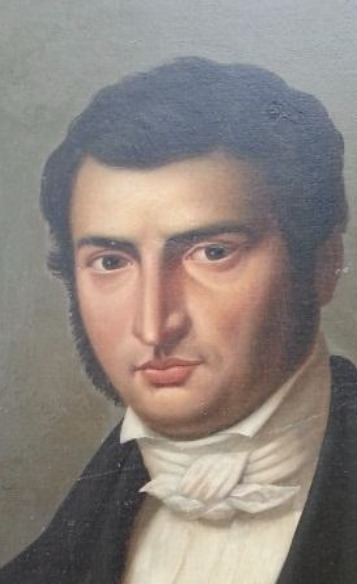
\includegraphics[width=0.88\linewidth,height=0.40\textheight,keepaspectratio]{genealogie/assets/galerie/portraits/portrait-55853aec3a8b761a1103.jpg}}
\par\vspace{0.10cm}
\galleryworktitle{Portrait de François Felix Berloty}
\galleryworkline{Source}{\href{https://www.geneanet.org/media/public/capture-d-ecran-2026-04-03-a-22-18-34-86290015}{Source en ligne}}
\end{minipage}
\par\vspace{0.30cm}
\noindent\setlength{\fboxsep}{6pt}\colorbox{GalleryCream}{
\parbox[t]{\dimexpr\linewidth-2\fboxsep-0.4cm\relax}{
\gallerysection{Citations dans l'ouvrage}
{\footnotesize\itshape\color{GalleryMuted} Aucune citation directement rattachée dans l'ouvrage.}
}
}
\vfill
\noindent\textcolor{GallerySand}{\rule{\textwidth}{0.6pt}}\par
{\scriptsize\color{GalleryMuted}Personnage cité dans les Mémoires de Benoît Coste}\par
\restoregeometry
\endgroup

\clearpage
\thispagestyle{plain}
\begingroup
\newgeometry{top=1.15cm,bottom=1.25cm,left=1.30cm,right=1.30cm}
\raggedbottom

\gallerypageheader
{\LARGE\bfseries\color{GalleryInk} Marie-Madeleine BRIASSON}\par
\vspace{0.12cm}
\noindent\textcolor{GallerySand}{\rule{\textwidth}{1.1pt}}\par
\vspace{0.15cm}
{\footnotesize\bfseries\color{GalleryMuted}\MakeUppercase{Relation avec Benoît Coste}}\par
{\large\color{GalleryBordeaux} Sa grand-mère}\par
\vspace{0.45cm}
\noindent\begin{minipage}[t]{0.52\textwidth}
\noindent\setlength{\fboxsep}{8pt}\colorbox{GalleryCream}{\parbox[t]{\dimexpr\linewidth-2\fboxsep\relax}{\galleryfact{Naissance}{8 septembre 1735 — Notre-Dame-de-la-Platière}
\galleryfact{Décès}{5 mars 1813 — Lyon}
\galleryfact{Profession}{Non renseignée}}}
\end{minipage}\hfill
\begin{minipage}[t]{0.43\textwidth}\centering
\setlength{\fboxsep}{4pt}\setlength{\fboxrule}{0.8pt}\fcolorbox{GalleryTerracotta}{white}{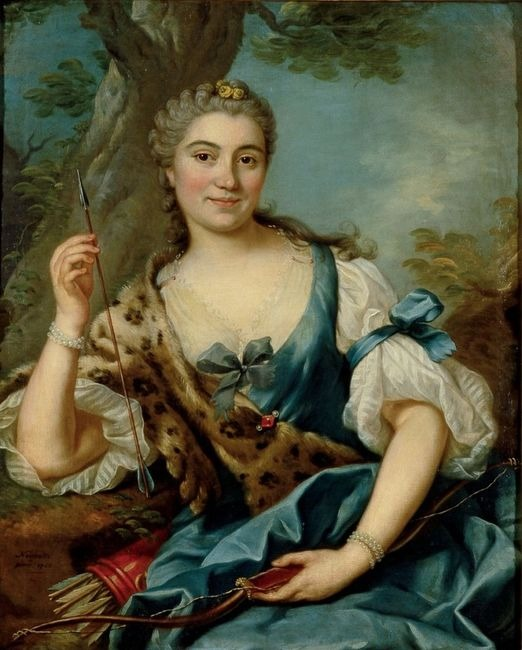
\includegraphics[width=0.88\linewidth,height=0.40\textheight,keepaspectratio]{genealogie/assets/galerie/portraits/portrait-c3fc93807db8aff73cc1.jpg}}
\par\vspace{0.10cm}
\galleryworktitle{Marie-Madeleine JORDAN en Diane}
\galleryworkline{Date}{1760}
\galleryworkline{Artiste}{Nonnotte Donat}
\galleryworkline{Source}{\href{https://collections.mba-lyon.fr/fr/notice/1970-535-marie-madeleine-jordan-en-diane-0399dacd-af80-45e7-a07f-bd2892db3c5b}{Musée des Beaux Arts de Lyon - Inventaire 1970-535}}
\end{minipage}
\par\vspace{0.30cm}
\noindent\setlength{\fboxsep}{6pt}\colorbox{GalleryCream}{
\parbox[t]{\dimexpr\linewidth-2\fboxsep-0.4cm\relax}{
\gallerysection{Citations dans l'ouvrage}
{\scriptsize\itshape\color{GalleryMuted} Benoît Coste — Mes souvenirs de soixante ans}\par\vspace{0.10cm}
{\footnotesize\begin{itemize}\setlength{\itemsep}{0pt}\setlength{\topsep}{1pt}\setlength{\parsep}{0pt}\setlength{\parskip}{0pt}
\item Chapitre 18 — p. 138 — \textit{« Ma respectable et vénérée Grand'mère avait été atteinte successivement... de deux attaques d'apoplexie ; deux mois après, il en survint une troisième... Ce fut le 5 mars 1813 que ce sacrifice nous fut imposé »}
\end{itemize}}
}
}
\vfill
\noindent\textcolor{GallerySand}{\rule{\textwidth}{0.6pt}}\par
{\scriptsize\color{GalleryMuted}Personnage cité dans les Mémoires de Benoît Coste}\par
\restoregeometry
\endgroup

\clearpage
\thispagestyle{plain}
\begingroup
\newgeometry{top=1.15cm,bottom=1.25cm,left=1.30cm,right=1.30cm}
\raggedbottom

\gallerypageheader
{\LARGE\bfseries\color{GalleryInk} Pierre François COLOMB DE GAST}\par
\vspace{0.12cm}
\noindent\textcolor{GallerySand}{\rule{\textwidth}{1.1pt}}\par
\vspace{0.15cm}
{\footnotesize\bfseries\color{GalleryMuted}\MakeUppercase{Relation avec Benoît Coste}}\par
{\large\color{GalleryBordeaux} Le père de son épouse Joséphine}\par
\vspace{0.45cm}
\noindent\setlength{\fboxsep}{8pt}\colorbox{GalleryCream}{\parbox[t]{\dimexpr\linewidth-2\fboxsep\relax}{\galleryfact{Naissance}{22 mai 1754 — Saint-Étienne}
\galleryfact{Décès}{21 septembre 1831 — Marlhes}
\gallerysection{Profession}
\small\begin{itemize}\setlength{\itemsep}{0pt}\setlength{\topsep}{2pt}\setlength{\parsep}{0pt}\setlength{\parskip}{0pt}
\item Député à l'Assemblée législative
\item Avocat au Parlement ; juge de paix élu de Saint-Chamond ; juge de paix de Marlhes et Saint-Genest-Malifaux ; membre du conseil général.
\end{itemize}}}
\par\vspace{0.40cm}
\begin{minipage}[t]{0.475\linewidth}\centering
\setlength{\fboxsep}{4pt}\setlength{\fboxrule}{0.8pt}\fcolorbox{GalleryTerracotta}{white}{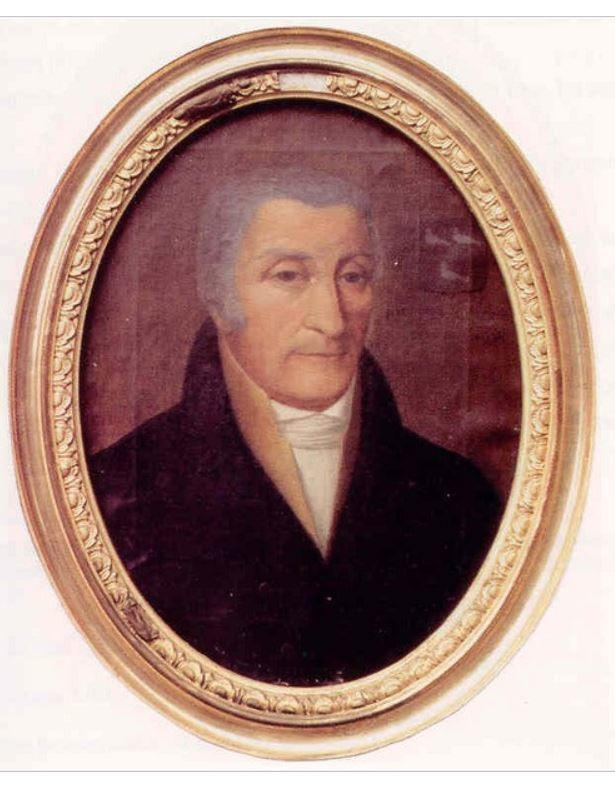
\includegraphics[width=0.88\linewidth,height=0.19\textheight,keepaspectratio]{genealogie/assets/galerie/portraits/portrait-226491f86cd7f9c43a5f.jpg}}
\par\vspace{0.10cm}
\galleryworktitle{Portrait de Pierre François Colomb}
\galleryworkline{Source}{\href{https://www.geneanet.org/media/public/pierre-francois-colomb-de-hauteville-397199}{Source en ligne}}
\end{minipage}\hfill\begin{minipage}[t]{0.475\linewidth}\centering
\setlength{\fboxsep}{4pt}\setlength{\fboxrule}{0.8pt}\fcolorbox{GalleryTerracotta}{white}{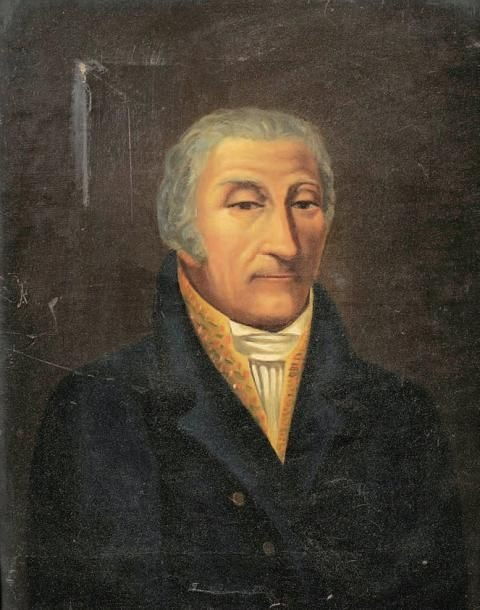
\includegraphics[width=0.88\linewidth,height=0.19\textheight,keepaspectratio]{genealogie/assets/galerie/portraits/portrait-41ef4bf090726a0f1161.jpg}}
\par\vspace{0.10cm}
\galleryworktitle{Portrait de Pierre François Colomb de Gaste — École française du XIXème siècle — Oger \& Blanchet, lot 61}
\galleryworkline{Artiste}{École française du XIXème siècle}
\galleryworkline{Source}{\href{https://www.ogerblanchet.fr/en/lot/10084/1866313-ecole-francaise-du-xixeme-siecle-portrait-de-pierre-francois}{Oger \& Blanchet — Vente « Tableaux, meubles et objets d’art... », Drouot-Richelieu, salle 7, 16 mai 2011, lot 61}}
\end{minipage}
\par\vspace{0.30cm}
\noindent\setlength{\fboxsep}{6pt}\colorbox{GalleryCream}{
\parbox[t]{\dimexpr\linewidth-2\fboxsep-0.4cm\relax}{
\gallerysection{Citations dans l'ouvrage}
{\scriptsize\itshape\color{GalleryMuted} Benoît Coste — Mes souvenirs de soixante ans}\par\vspace{0.10cm}
{\footnotesize\begin{itemize}\setlength{\itemsep}{0pt}\setlength{\topsep}{1pt}\setlength{\parsep}{0pt}\setlength{\parskip}{0pt}
\item Chapitre 22 — p. 175 — \textit{« monsieur Colomb de Gast est mon beau-père. »}
\item Chapitre 30 — p. 246 — \textit{« le 21 septembre 1831, entouré comme les patriarches de l’ancienne loi, de tous ses enfants, il rend son âme à Dieu »}
\end{itemize}}
}
}
\vfill
\noindent\textcolor{GallerySand}{\rule{\textwidth}{0.6pt}}\par
{\scriptsize\color{GalleryMuted}Personnage cité dans les Mémoires de Benoît Coste}\par
\restoregeometry
\endgroup

\clearpage
\thispagestyle{plain}
\begingroup
\newgeometry{top=1.15cm,bottom=1.25cm,left=1.30cm,right=1.30cm}
\raggedbottom

\gallerypageheader
{\LARGE\bfseries\color{GalleryInk} \underline{Adélaïde} COSTE}\par
\vspace{0.12cm}
\noindent\textcolor{GallerySand}{\rule{\textwidth}{1.1pt}}\par
\vspace{0.15cm}
{\footnotesize\bfseries\color{GalleryMuted}\MakeUppercase{Relation avec Benoît Coste}}\par
{\large\color{GalleryBordeaux} Sa sœur}\par
\vspace{0.45cm}
\noindent\begin{minipage}[t]{0.52\textwidth}
\noindent\setlength{\fboxsep}{8pt}\colorbox{GalleryCream}{\parbox[t]{\dimexpr\linewidth-2\fboxsep\relax}{\galleryfact{Naissance}{Non renseignée}
\galleryfact{Décès}{1836}
\galleryfact{Profession}{Non renseignée}}}
\end{minipage}\hfill
\begin{minipage}[t]{0.43\textwidth}\centering
\setlength{\fboxsep}{0pt}\setlength{\fboxrule}{0.8pt}
\fcolorbox{GallerySand}{GalleryCream}{
\parbox[c][0.50\textheight][c]{0.90\linewidth}{\centering
{\fontsize{48}{54}\selectfont\bfseries\color{GalleryBordeaux} AC}\par\medskip
{\small\color{GalleryMuted}Portrait non disponible}\par}}
\end{minipage}
\par\vspace{0.30cm}
\noindent\setlength{\fboxsep}{6pt}\colorbox{GalleryCream}{
\parbox[t]{\dimexpr\linewidth-2\fboxsep-0.4cm\relax}{
\gallerysection{Citations dans l'ouvrage}
{\scriptsize\itshape\color{GalleryMuted} Benoît Coste — Mes souvenirs de soixante ans}\par\vspace{0.10cm}
{\footnotesize\begin{itemize}\setlength{\itemsep}{0pt}\setlength{\topsep}{1pt}\setlength{\parsep}{0pt}\setlength{\parskip}{0pt}
\item Chapitre 1 — p. 6 — \textit{« J'avais trois sœurs, toutes mes aînées : Madeleine, Catherine et Adélaïde. »}
\item Chapitre 3 — p. 22 — \textit{« Mes sœurs Catherine et Adélaïde, qui n'avaient pas encore été confirmées, le furent en même temps. »}
\item Chapitre 15 — p. 107 — \textit{« mariage de ma sœur cadette. Elle épousa au mois de février 1806, Monsieur Franchet, docteur en médecine. »}
\item Chapitre 35 — p. 282 — \textit{« 1836 – Mort de ma sœur Franchet... la perte de ma bonne sœur Adélaïde Franchet. »}
\end{itemize}}
}
}
\vfill
\noindent\textcolor{GallerySand}{\rule{\textwidth}{0.6pt}}\par
{\scriptsize\color{GalleryMuted}Personnage cité dans les Mémoires de Benoît Coste}\par
\restoregeometry
\endgroup

\clearpage
\thispagestyle{plain}
\begingroup
\newgeometry{top=1.15cm,bottom=1.25cm,left=1.30cm,right=1.30cm}
\raggedbottom

\gallerypageheader
{\LARGE\bfseries\color{GalleryInk} Benoit COSTE}\par
\vspace{0.12cm}
\noindent\textcolor{GallerySand}{\rule{\textwidth}{1.1pt}}\par
\vspace{0.15cm}
{\footnotesize\bfseries\color{GalleryMuted}\MakeUppercase{Relation avec Benoît Coste}}\par
{\large\color{GalleryBordeaux} Son grand-père}\par
\vspace{0.45cm}
\noindent\begin{minipage}[t]{0.52\textwidth}
\noindent\setlength{\fboxsep}{8pt}\colorbox{GalleryCream}{\parbox[t]{\dimexpr\linewidth-2\fboxsep\relax}{\galleryfact{Naissance}{17 octobre 1712 — Lyon}
\galleryfact{Décès}{8 février 1789 — Lyon}
\gallerysection{Profession}
\small\begin{itemize}\setlength{\itemsep}{0pt}\setlength{\topsep}{2pt}\setlength{\parsep}{0pt}\setlength{\parskip}{0pt}
\item Recteur de la Charité
\item Échevin
\item Recteur de l'hotel Dieu
\item Marchand de Soie
\end{itemize}}}
\end{minipage}\hfill
\begin{minipage}[t]{0.43\textwidth}\centering
\setlength{\fboxsep}{4pt}\setlength{\fboxrule}{0.8pt}\fcolorbox{GalleryTerracotta}{white}{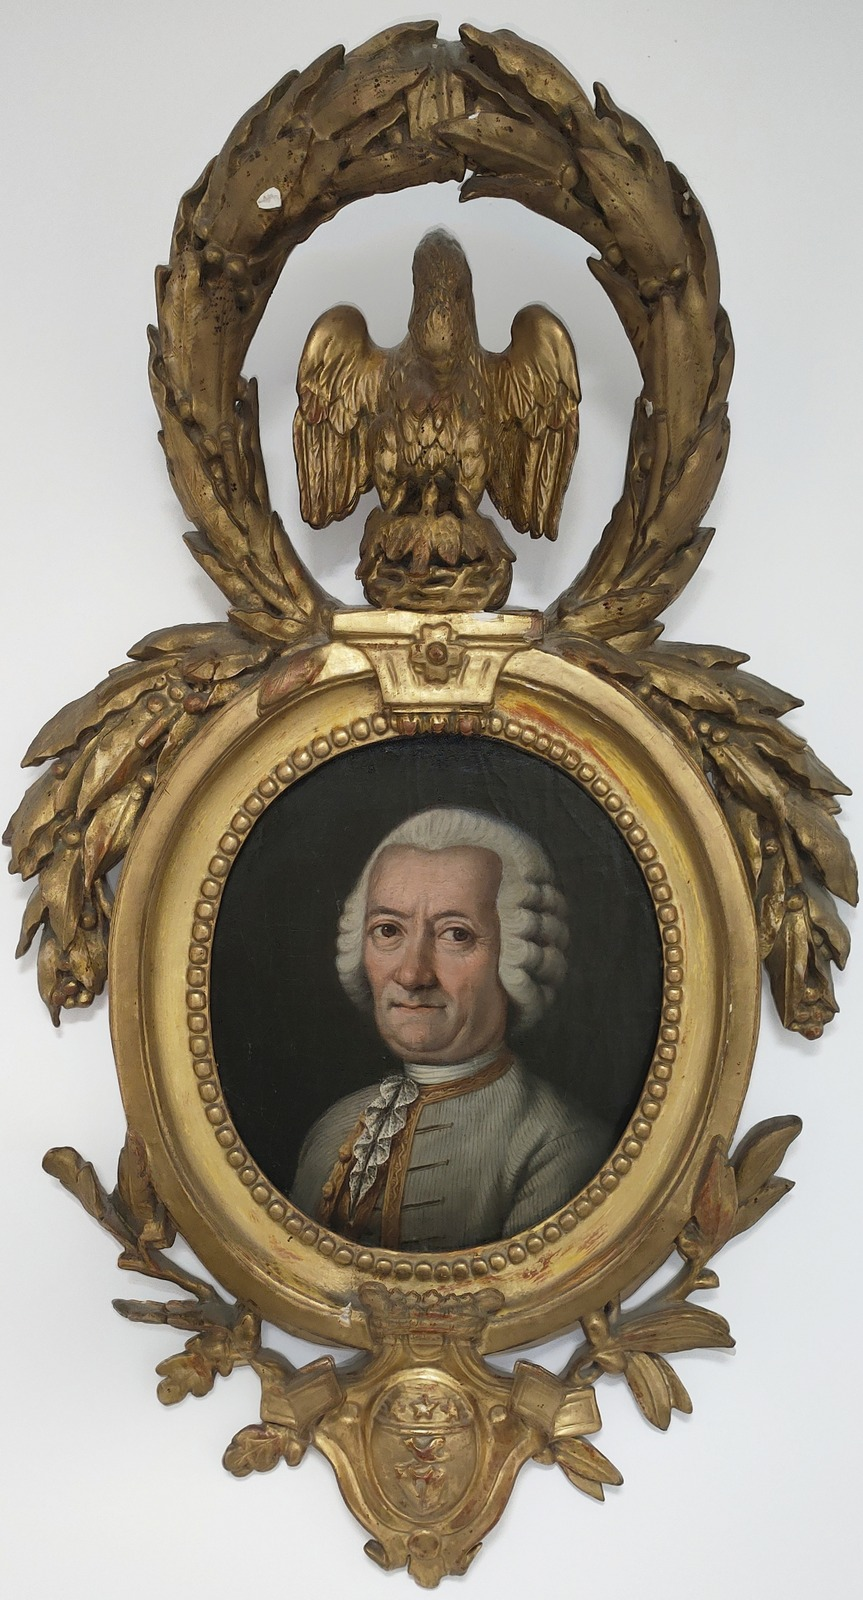
\includegraphics[width=0.88\linewidth,height=0.40\textheight,keepaspectratio]{genealogie/assets/galerie/portraits/portrait-eb55b553ec501ead16b6.jpg}}
\par\vspace{0.10cm}
\galleryworktitle{Portrait de Benoit Coste — vue complète du cadre}
\galleryworkline{Source}{Portrait propriété de la Famille.}
\end{minipage}
\par\vspace{0.30cm}
\noindent\setlength{\fboxsep}{6pt}\colorbox{GalleryCream}{
\parbox[t]{\dimexpr\linewidth-2\fboxsep-0.4cm\relax}{
\gallerysection{Citations dans l'ouvrage}
{\scriptsize\itshape\color{GalleryMuted} Benoît Coste — Mes souvenirs de soixante ans}\par\vspace{0.10cm}
{\footnotesize\begin{itemize}\setlength{\itemsep}{0pt}\setlength{\topsep}{1pt}\setlength{\parsep}{0pt}\setlength{\parskip}{0pt}
\item Chapitre 2 — p. 16 — \textit{« Mon grand père paternel était mort en 1793 »}
\end{itemize}}
}
}
\vfill
\noindent\textcolor{GallerySand}{\rule{\textwidth}{0.6pt}}\par
{\scriptsize\color{GalleryMuted}Personnage cité dans les Mémoires de Benoît Coste}\par
\restoregeometry
\endgroup

\clearpage
\thispagestyle{plain}
\begingroup
\newgeometry{top=1.15cm,bottom=1.25cm,left=1.30cm,right=1.30cm}
\raggedbottom

\gallerypageheader
{\LARGE\bfseries\color{GalleryInk} Catherine COSTE}\par
\vspace{0.12cm}
\noindent\textcolor{GallerySand}{\rule{\textwidth}{1.1pt}}\par
\vspace{0.15cm}
{\footnotesize\bfseries\color{GalleryMuted}\MakeUppercase{Relation avec Benoît Coste}}\par
{\large\color{GalleryBordeaux} Sa sœur}\par
\vspace{0.45cm}
\noindent\begin{minipage}[t]{0.52\textwidth}
\noindent\setlength{\fboxsep}{8pt}\colorbox{GalleryCream}{\parbox[t]{\dimexpr\linewidth-2\fboxsep\relax}{\galleryfact{Naissance}{Non renseignée}
\galleryfact{Décès}{Non renseignée}
\gallerysection{Profession}
\small\begin{itemize}\setlength{\itemsep}{0pt}\setlength{\topsep}{2pt}\setlength{\parsep}{0pt}\setlength{\parskip}{0pt}
\item Religieuse de Saint Michel
\end{itemize}}}
\end{minipage}\hfill
\begin{minipage}[t]{0.43\textwidth}\centering
\setlength{\fboxsep}{0pt}\setlength{\fboxrule}{0.8pt}
\fcolorbox{GallerySand}{GalleryCream}{
\parbox[c][0.50\textheight][c]{0.90\linewidth}{\centering
{\fontsize{48}{54}\selectfont\bfseries\color{GalleryBordeaux} CC}\par\medskip
{\small\color{GalleryMuted}Portrait non disponible}\par}}
\end{minipage}
\par\vspace{0.30cm}
\noindent\setlength{\fboxsep}{6pt}\colorbox{GalleryCream}{
\parbox[t]{\dimexpr\linewidth-2\fboxsep-0.4cm\relax}{
\gallerysection{Citations dans l'ouvrage}
{\scriptsize\itshape\color{GalleryMuted} Benoît Coste — Mes souvenirs de soixante ans}\par\vspace{0.10cm}
{\footnotesize\begin{itemize}\setlength{\itemsep}{0pt}\setlength{\topsep}{1pt}\setlength{\parsep}{0pt}\setlength{\parskip}{0pt}
\item Chapitre 1 — p. 6 — \textit{« J'avais trois sœurs, toutes mes aînées : Madeleine, Catherine et Adélaïde. »}
\item Chapitre 3 — p. 22 — \textit{« Mes sœurs Catherine et Adélaïde, qui n'avaient pas encore été confirmées, le furent en même temps. »}
\item Chapitre 16 — p. 117 — \textit{« trois semaines à peu près après notre union, notre sœur s'arrache à notre tendre amitié... part pour Paris et va se renfermer au monastère des dames St Michel. »}
\end{itemize}}
}
}
\vfill
\noindent\textcolor{GallerySand}{\rule{\textwidth}{0.6pt}}\par
{\scriptsize\color{GalleryMuted}Personnage cité dans les Mémoires de Benoît Coste}\par
\restoregeometry
\endgroup

\clearpage
\thispagestyle{plain}
\begingroup
\newgeometry{top=1.15cm,bottom=1.25cm,left=1.30cm,right=1.30cm}
\raggedbottom

\gallerypageheader
{\LARGE\bfseries\color{GalleryInk} Madeleine COSTE}\par
\vspace{0.12cm}
\noindent\textcolor{GallerySand}{\rule{\textwidth}{1.1pt}}\par
\vspace{0.15cm}
{\footnotesize\bfseries\color{GalleryMuted}\MakeUppercase{Relation avec Benoît Coste}}\par
{\large\color{GalleryBordeaux} Sa sœur}\par
\vspace{0.45cm}
\noindent\begin{minipage}[t]{0.52\textwidth}
\noindent\setlength{\fboxsep}{8pt}\colorbox{GalleryCream}{\parbox[t]{\dimexpr\linewidth-2\fboxsep\relax}{\galleryfact{Naissance}{3 avril 1775}
\galleryfact{Décès}{27 novembre 1854}
\galleryfact{Profession}{Non renseignée}}}
\end{minipage}\hfill
\begin{minipage}[t]{0.43\textwidth}\centering
\setlength{\fboxsep}{0pt}\setlength{\fboxrule}{0.8pt}
\fcolorbox{GallerySand}{GalleryCream}{
\parbox[c][0.50\textheight][c]{0.90\linewidth}{\centering
{\fontsize{48}{54}\selectfont\bfseries\color{GalleryBordeaux} MC}\par\medskip
{\small\color{GalleryMuted}Portrait non disponible}\par}}
\end{minipage}
\par\vspace{0.30cm}
\noindent\setlength{\fboxsep}{6pt}\colorbox{GalleryCream}{
\parbox[t]{\dimexpr\linewidth-2\fboxsep-0.4cm\relax}{
\gallerysection{Citations dans l'ouvrage}
{\scriptsize\itshape\color{GalleryMuted} Benoît Coste — Mes souvenirs de soixante ans}\par\vspace{0.10cm}
{\footnotesize\begin{itemize}\setlength{\itemsep}{0pt}\setlength{\topsep}{1pt}\setlength{\parsep}{0pt}\setlength{\parskip}{0pt}
\item Chapitre 1 — p. 6 — \textit{« J'avais trois sœurs, toutes mes aînées : Madeleine, Catherine et Adélaïde. »}
\end{itemize}}
}
}
\vfill
\noindent\textcolor{GallerySand}{\rule{\textwidth}{0.6pt}}\par
{\scriptsize\color{GalleryMuted}Personnage cité dans les Mémoires de Benoît Coste}\par
\restoregeometry
\endgroup

\clearpage
\thispagestyle{plain}
\begingroup
\newgeometry{top=1.15cm,bottom=1.25cm,left=1.30cm,right=1.30cm}
\raggedbottom

\gallerypageheader
{\LARGE\bfseries\color{GalleryInk} Marie COSTE}\par
\vspace{0.12cm}
\noindent\textcolor{GallerySand}{\rule{\textwidth}{1.1pt}}\par
\vspace{0.15cm}
{\footnotesize\bfseries\color{GalleryMuted}\MakeUppercase{Relation avec Benoît Coste}}\par
{\large\color{GalleryBordeaux} Sa petite-fille}\par
\vspace{0.45cm}
\noindent\begin{minipage}[t]{0.52\textwidth}
\noindent\setlength{\fboxsep}{8pt}\colorbox{GalleryCream}{\parbox[t]{\dimexpr\linewidth-2\fboxsep\relax}{\galleryfact{Naissance}{Non renseignée}
\galleryfact{Décès}{Non renseignée}
\galleryfact{Profession}{Non renseignée}}}
\end{minipage}\hfill
\begin{minipage}[t]{0.43\textwidth}\centering
\setlength{\fboxsep}{0pt}\setlength{\fboxrule}{0.8pt}
\fcolorbox{GallerySand}{GalleryCream}{
\parbox[c][0.50\textheight][c]{0.90\linewidth}{\centering
{\fontsize{48}{54}\selectfont\bfseries\color{GalleryBordeaux} MC}\par\medskip
{\small\color{GalleryMuted}Portrait non disponible}\par}}
\end{minipage}
\par\vspace{0.30cm}
\noindent\setlength{\fboxsep}{6pt}\colorbox{GalleryCream}{
\parbox[t]{\dimexpr\linewidth-2\fboxsep-0.4cm\relax}{
\gallerysection{Citations dans l'ouvrage}
{\footnotesize\itshape\color{GalleryMuted} Aucune citation directement rattachée dans l'ouvrage.}
}
}
\vfill
\noindent\textcolor{GallerySand}{\rule{\textwidth}{0.6pt}}\par
{\scriptsize\color{GalleryMuted}Personnage cité dans les Mémoires de Benoît Coste}\par
\restoregeometry
\endgroup

\clearpage
\thispagestyle{plain}
\begingroup
\newgeometry{top=1.15cm,bottom=1.25cm,left=1.30cm,right=1.30cm}
\raggedbottom

\gallerypageheader
{\LARGE\bfseries\color{GalleryInk} Marie Antoinette GUERIN}\par
\vspace{0.12cm}
\noindent\textcolor{GallerySand}{\rule{\textwidth}{1.1pt}}\par
\vspace{0.15cm}
{\footnotesize\bfseries\color{GalleryMuted}\MakeUppercase{Relation avec Benoît Coste}}\par
{\large\color{GalleryBordeaux} La mère de son épouse Joséphine}\par
\vspace{0.45cm}
\noindent\setlength{\fboxsep}{8pt}\colorbox{GalleryCream}{\parbox[t]{\dimexpr\linewidth-2\fboxsep\relax}{\galleryfact{Naissance}{25 juin 1762 — Saint-Chamond}
\galleryfact{Décès}{24 février 1831 — St Sauveur en Rue}
\galleryfact{Profession}{Non renseignée}}}
\par\vspace{0.40cm}
\begin{minipage}[t]{0.475\linewidth}\centering
\setlength{\fboxsep}{4pt}\setlength{\fboxrule}{0.8pt}\fcolorbox{GalleryTerracotta}{white}{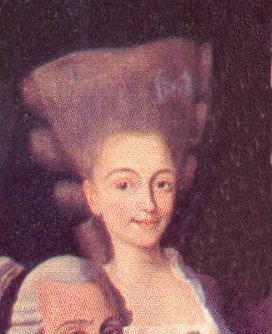
\includegraphics[width=0.88\linewidth,height=0.19\textheight,keepaspectratio]{genealogie/assets/galerie/portraits/portrait-10cfc5bd785558e62195.jpg}}
\par\vspace{0.10cm}
\galleryworktitle{Portrait de Marie Antoinette Guerin}
\galleryworkline{Source}{Non renseignée}
\end{minipage}\hfill\begin{minipage}[t]{0.475\linewidth}\centering
\setlength{\fboxsep}{4pt}\setlength{\fboxrule}{0.8pt}\fcolorbox{GalleryTerracotta}{white}{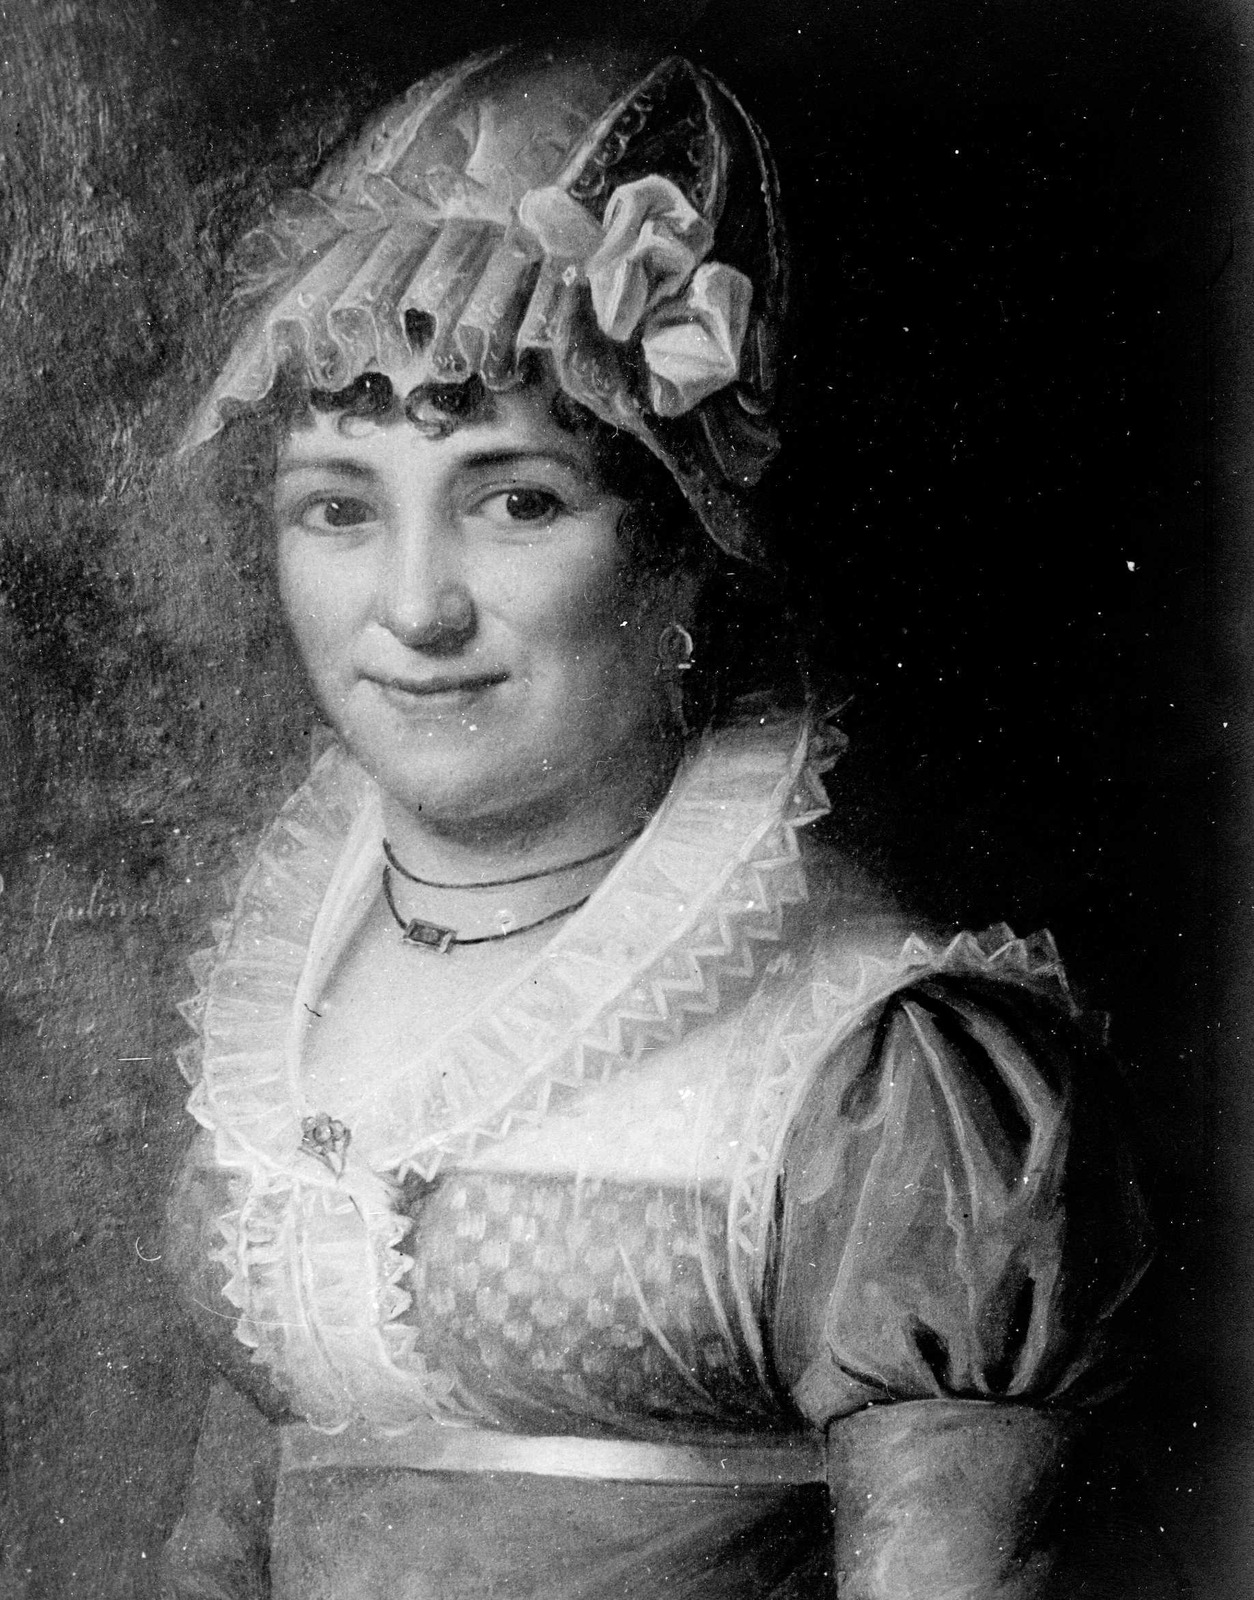
\includegraphics[width=0.88\linewidth,height=0.19\textheight,keepaspectratio]{genealogie/assets/galerie/portraits/portrait-ac75345f83c41ac14737.jpg}}
\par\vspace{0.10cm}
\galleryworktitle{Portrait de Marie Antoinette Guerin}
\galleryworkline{Source}{\href{https://www.geneanet.org/media/public/35-15792018}{Source en ligne}}
\end{minipage}
\par\vspace{0.30cm}
\noindent\setlength{\fboxsep}{6pt}\colorbox{GalleryCream}{
\parbox[t]{\dimexpr\linewidth-2\fboxsep-0.4cm\relax}{
\gallerysection{Citations dans l'ouvrage}
{\scriptsize\itshape\color{GalleryMuted} Benoît Coste — Mes souvenirs de soixante ans}\par\vspace{0.10cm}
{\footnotesize\begin{itemize}\setlength{\itemsep}{0pt}\setlength{\topsep}{1pt}\setlength{\parsep}{0pt}\setlength{\parskip}{0pt}
\item Chapitre 22 — p. 175 — \textit{« Madame, qui est une demoiselle Guérin ; elle m’expliqua qu’elle était de St Chamond »}
\item Chapitre 30 — p. 244 — \textit{« Ma belle-mère, nous fut enlevée en quelques heures, le 24 février 1831 »}
\end{itemize}}
}
}
\vfill
\noindent\textcolor{GallerySand}{\rule{\textwidth}{0.6pt}}\par
{\scriptsize\color{GalleryMuted}Personnage cité dans les Mémoires de Benoît Coste}\par
\restoregeometry
\endgroup

\clearpage
\thispagestyle{plain}
\begingroup
\newgeometry{top=1.15cm,bottom=1.25cm,left=1.30cm,right=1.30cm}
\raggedbottom

\gallerypageheader
{\LARGE\bfseries\color{GalleryInk} Antoine Henry JORDAN}\par
\vspace{0.12cm}
\noindent\textcolor{GallerySand}{\rule{\textwidth}{1.1pt}}\par
\vspace{0.15cm}
{\footnotesize\bfseries\color{GalleryMuted}\MakeUppercase{Relation avec Benoît Coste}}\par
{\large\color{GalleryBordeaux} Son grand-père}\par
\vspace{0.45cm}
\noindent\setlength{\fboxsep}{8pt}\colorbox{GalleryCream}{\parbox[t]{\dimexpr\linewidth-2\fboxsep\relax}{\galleryfact{Naissance}{3 janvier 1725 — Lyon}
\galleryfact{Décès}{31 janvier 1794 — Lyon}
\gallerysection{Profession}
\small\begin{itemize}\setlength{\itemsep}{0pt}\setlength{\topsep}{2pt}\setlength{\parsep}{0pt}\setlength{\parskip}{0pt}
\item Échevin
\item Marchand de Soie
\item Banquier
\end{itemize}}}
\par\vspace{0.40cm}
\begin{minipage}[t]{0.475\linewidth}\centering
\setlength{\fboxsep}{4pt}\setlength{\fboxrule}{0.8pt}\fcolorbox{GalleryTerracotta}{white}{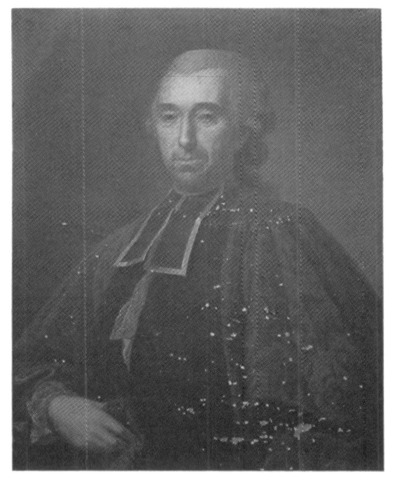
\includegraphics[width=0.88\linewidth,height=0.19\textheight,keepaspectratio]{genealogie/assets/galerie/portraits/portrait-4ba23a6053af8733b287.jpg}}
\par\vspace{0.10cm}
\galleryworktitle{Illustration 19 — portrait d’Antoine-Henri Jordan — reproduction Persée}
\galleryworkline{Source}{\href{https://www.persee.fr/renderIllustration/bmml\_0521-7032\_1993\_num\_1993\_3\_T1\_0083\_0000\_2.png}{Source en ligne}}
\end{minipage}\hfill\begin{minipage}[t]{0.475\linewidth}\centering
\setlength{\fboxsep}{4pt}\setlength{\fboxrule}{0.8pt}\fcolorbox{GalleryTerracotta}{white}{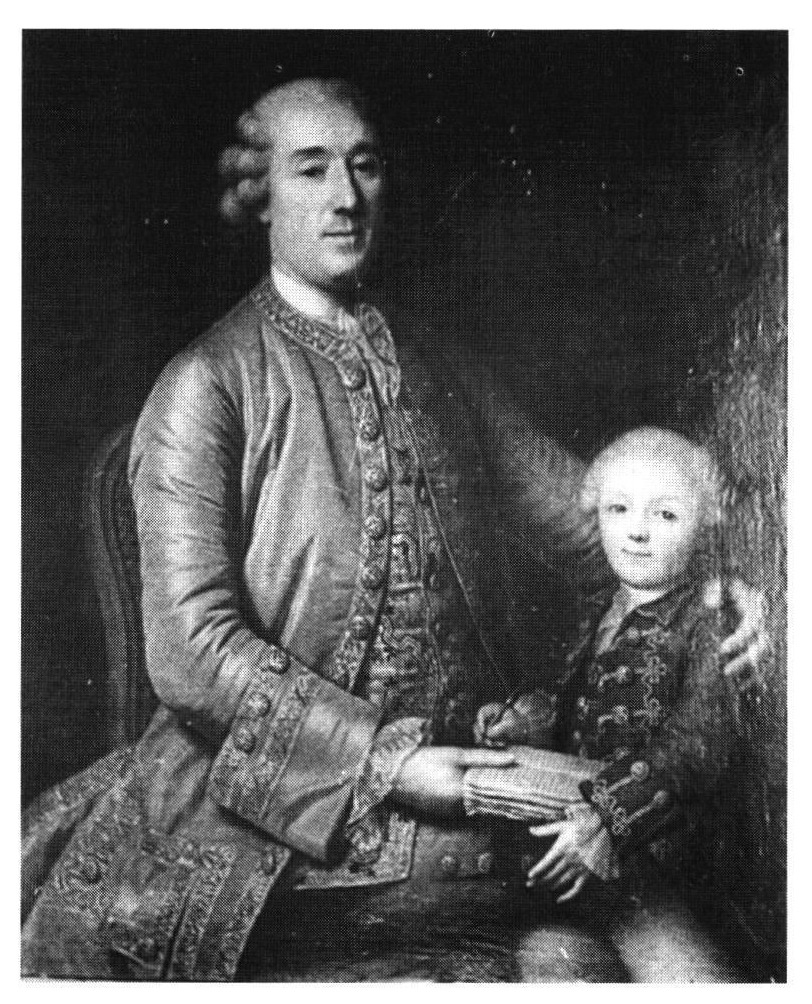
\includegraphics[width=0.88\linewidth,height=0.19\textheight,keepaspectratio]{genealogie/assets/galerie/portraits/portrait-cbd2d207501bc80d7213.jpg}}
\par\vspace{0.10cm}
\galleryworktitle{Double portraits de Antoine Henri I Jordan et son fils Antoine Henri II}
\galleryworkline{Artiste}{Donat Nonotte}
\galleryworkline{Source}{\href{https://books.openedition.org/efr/2016}{Collection privée}}
\end{minipage}
\par\vspace{0.30cm}
\noindent\setlength{\fboxsep}{6pt}\colorbox{GalleryCream}{
\parbox[t]{\dimexpr\linewidth-2\fboxsep-0.4cm\relax}{
\gallerysection{Citations dans l'ouvrage}
{\scriptsize\itshape\color{GalleryMuted} Benoît Coste — Mes souvenirs de soixante ans}\par\vspace{0.10cm}
{\footnotesize\begin{itemize}\setlength{\itemsep}{0pt}\setlength{\topsep}{1pt}\setlength{\parsep}{0pt}\setlength{\parskip}{0pt}
\item Chapitre 1 — p. 6 — \textit{« Ma mère, aussi fille d'un marchand de soie »}
\item Chapitre 2 — p. 16 — \textit{« Pendant cette triste époque, nous avons perdu trois parents, parmi lesquels mon grand-père maternel. »}
\end{itemize}}
}
}
\vfill
\noindent\textcolor{GallerySand}{\rule{\textwidth}{0.6pt}}\par
{\scriptsize\color{GalleryMuted}Personnage cité dans les Mémoires de Benoît Coste}\par
\restoregeometry
\endgroup

\clearpage
\thispagestyle{plain}
\begingroup
\newgeometry{top=1.15cm,bottom=1.25cm,left=1.30cm,right=1.30cm}
\raggedbottom

\gallerypageheader
{\LARGE\bfseries\color{GalleryInk} Joseph-Antoine COLOMB DE GASTE}\par
\vspace{0.12cm}
\noindent\textcolor{GallerySand}{\rule{\textwidth}{1.1pt}}\par
\vspace{0.15cm}
{\footnotesize\bfseries\color{GalleryMuted}\MakeUppercase{Relation avec Benoît Coste}}\par
{\large\color{GalleryBordeaux} Son beau-frère}\par
\vspace{0.45cm}
\noindent\begin{minipage}[t]{0.52\textwidth}
\noindent\setlength{\fboxsep}{8pt}\colorbox{GalleryCream}{\parbox[t]{\dimexpr\linewidth-2\fboxsep\relax}{\galleryfact{Naissance}{12 juin 1789}
\galleryfact{Décès}{25 septembre 1859 — Le Coing}
\galleryfact{Profession}{Non renseignée}}}
\end{minipage}\hfill
\begin{minipage}[t]{0.43\textwidth}\centering
\setlength{\fboxsep}{0pt}\setlength{\fboxrule}{0.8pt}
\fcolorbox{GallerySand}{GalleryCream}{
\parbox[c][0.50\textheight][c]{0.90\linewidth}{\centering
{\fontsize{48}{54}\selectfont\bfseries\color{GalleryBordeaux} JC}\par\medskip
{\small\color{GalleryMuted}Portrait non disponible}\par}}
\end{minipage}
\par\vspace{0.30cm}
\noindent\setlength{\fboxsep}{6pt}\colorbox{GalleryCream}{
\parbox[t]{\dimexpr\linewidth-2\fboxsep-0.4cm\relax}{
\gallerysection{Citations dans l'ouvrage}
{\scriptsize\itshape\color{GalleryMuted} Benoît Coste — Mes souvenirs de soixante ans}\par\vspace{0.10cm}
{\footnotesize\begin{itemize}\setlength{\itemsep}{0pt}\setlength{\topsep}{1pt}\setlength{\parsep}{0pt}\setlength{\parskip}{0pt}
\item Chapitre 16 — p. 119 — \textit{« Votre oncle Colomb avait terminé ses études dans le courant de 1808... Il fut décidé à notre grande satisfaction qu'il logerait et mangerait à la maison. »}
\item Chapitre 18 — p. 138 — \textit{« Le 20 Mai de la même année votre oncle Colomb épousa Mademoiselle G..... »}
\end{itemize}}
}
}
\vfill
\noindent\textcolor{GallerySand}{\rule{\textwidth}{0.6pt}}\par
{\scriptsize\color{GalleryMuted}Personnage cité dans les Mémoires de Benoît Coste}\par
\restoregeometry
\endgroup

\clearpage
\thispagestyle{plain}
\begingroup
\newgeometry{top=1.15cm,bottom=1.25cm,left=1.30cm,right=1.30cm}
\raggedbottom

\gallerypageheader
{\LARGE\bfseries\color{GalleryInk} François Isaac COSTE}\par
\vspace{0.12cm}
\noindent\textcolor{GallerySand}{\rule{\textwidth}{1.1pt}}\par
\vspace{0.15cm}
{\footnotesize\bfseries\color{GalleryMuted}\MakeUppercase{Relation avec Benoît Coste}}\par
{\large\color{GalleryBordeaux} Son oncle}\par
\vspace{0.45cm}
\noindent\begin{minipage}[t]{0.52\textwidth}
\noindent\setlength{\fboxsep}{8pt}\colorbox{GalleryCream}{\parbox[t]{\dimexpr\linewidth-2\fboxsep\relax}{\galleryfact{Naissance}{1734}
\galleryfact{Décès}{1793}
\galleryfact{Profession}{Non renseignée}}}
\end{minipage}\hfill
\begin{minipage}[t]{0.43\textwidth}\centering
\setlength{\fboxsep}{0pt}\setlength{\fboxrule}{0.8pt}
\fcolorbox{GallerySand}{GalleryCream}{
\parbox[c][0.50\textheight][c]{0.90\linewidth}{\centering
{\fontsize{48}{54}\selectfont\bfseries\color{GalleryBordeaux} FC}\par\medskip
{\small\color{GalleryMuted}Portrait non disponible}\par}}
\end{minipage}
\par\vspace{0.30cm}
\noindent\setlength{\fboxsep}{6pt}\colorbox{GalleryCream}{
\parbox[t]{\dimexpr\linewidth-2\fboxsep-0.4cm\relax}{
\gallerysection{Citations dans l'ouvrage}
{\scriptsize\itshape\color{GalleryMuted} Benoît Coste — Mes souvenirs de soixante ans}\par\vspace{0.10cm}
{\footnotesize\begin{itemize}\setlength{\itemsep}{0pt}\setlength{\topsep}{1pt}\setlength{\parsep}{0pt}\setlength{\parskip}{0pt}
\item Chapitre 2 — p. 16 — \textit{« son frère aîné qui a, hélas, payé de sa tête sa fatale sécurité. »}
\end{itemize}}
}
}
\vfill
\noindent\textcolor{GallerySand}{\rule{\textwidth}{0.6pt}}\par
{\scriptsize\color{GalleryMuted}Personnage cité dans les Mémoires de Benoît Coste}\par
\restoregeometry
\endgroup

\clearpage
\thispagestyle{plain}
\begingroup
\newgeometry{top=1.15cm,bottom=1.25cm,left=1.30cm,right=1.30cm}
\raggedbottom

\gallerypageheader
{\LARGE\bfseries\color{GalleryInk} Amélie DE COLOMB}\par
\vspace{0.12cm}
\noindent\textcolor{GallerySand}{\rule{\textwidth}{1.1pt}}\par
\vspace{0.15cm}
{\footnotesize\bfseries\color{GalleryMuted}\MakeUppercase{Relation avec Benoît Coste}}\par
{\large\color{GalleryBordeaux} Sa belle-sœur Amélie Colomb}\par
\vspace{0.45cm}
\noindent\begin{minipage}[t]{0.52\textwidth}
\noindent\setlength{\fboxsep}{8pt}\colorbox{GalleryCream}{\parbox[t]{\dimexpr\linewidth-2\fboxsep\relax}{\galleryfact{Naissance}{1793}
\galleryfact{Décès}{Non renseignée}
\galleryfact{Profession}{Non renseignée}}}
\end{minipage}\hfill
\begin{minipage}[t]{0.43\textwidth}\centering
\setlength{\fboxsep}{4pt}\setlength{\fboxrule}{0.8pt}\fcolorbox{GalleryTerracotta}{white}{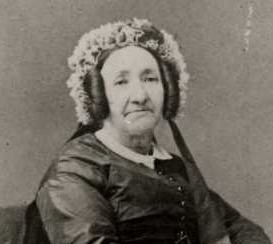
\includegraphics[width=0.88\linewidth,height=0.40\textheight,keepaspectratio]{genealogie/assets/galerie/portraits/portrait-1ee70a0cf89e118f9978.jpg}}
\par\vspace{0.10cm}
\galleryworktitle{Portrait d'Amélie de Colomb}
\galleryworkline{Source}{\href{https://gw.geneanet.org/soniaberg?lang=fr\&n=colomb+de+gast\&p=marie+antoinette+amelie\&type=fiche}{Source en ligne}}
\end{minipage}
\par\vspace{0.30cm}
\noindent\setlength{\fboxsep}{6pt}\colorbox{GalleryCream}{
\parbox[t]{\dimexpr\linewidth-2\fboxsep-0.4cm\relax}{
\gallerysection{Citations dans l'ouvrage}
{\scriptsize\itshape\color{GalleryMuted} Benoît Coste — Mes souvenirs de soixante ans}\par\vspace{0.10cm}
{\footnotesize\begin{itemize}\setlength{\itemsep}{0pt}\setlength{\topsep}{1pt}\setlength{\parsep}{0pt}\setlength{\parskip}{0pt}
\item Chapitre 23 — p. 181 — \textit{« celui du mariage de ma belle-sœur Amélie Colomb ; elle épousa M. Adrien Neyrat »}
\end{itemize}}
}
}
\vfill
\noindent\textcolor{GallerySand}{\rule{\textwidth}{0.6pt}}\par
{\scriptsize\color{GalleryMuted}Personnage cité dans les Mémoires de Benoît Coste}\par
\restoregeometry
\endgroup

\clearpage
\thispagestyle{plain}
\begingroup
\newgeometry{top=1.15cm,bottom=1.25cm,left=1.30cm,right=1.30cm}
\raggedbottom

\gallerypageheader
{\LARGE\bfseries\color{GalleryInk} Claude Joseph FRANCHET}\par
\vspace{0.12cm}
\noindent\textcolor{GallerySand}{\rule{\textwidth}{1.1pt}}\par
\vspace{0.15cm}
{\footnotesize\bfseries\color{GalleryMuted}\MakeUppercase{Relation avec Benoît Coste}}\par
{\large\color{GalleryBordeaux} Le mari de sa sœur Adélaïde Coste}\par
\vspace{0.45cm}
\noindent\begin{minipage}[t]{0.52\textwidth}
\noindent\setlength{\fboxsep}{8pt}\colorbox{GalleryCream}{\parbox[t]{\dimexpr\linewidth-2\fboxsep\relax}{\galleryfact{Naissance}{Non renseignée}
\galleryfact{Décès}{1813}
\galleryfact{Profession}{Non renseignée}}}
\end{minipage}\hfill
\begin{minipage}[t]{0.43\textwidth}\centering
\setlength{\fboxsep}{0pt}\setlength{\fboxrule}{0.8pt}
\fcolorbox{GallerySand}{GalleryCream}{
\parbox[c][0.50\textheight][c]{0.90\linewidth}{\centering
{\fontsize{48}{54}\selectfont\bfseries\color{GalleryBordeaux} CF}\par\medskip
{\small\color{GalleryMuted}Portrait non disponible}\par}}
\end{minipage}
\par\vspace{0.30cm}
\noindent\setlength{\fboxsep}{6pt}\colorbox{GalleryCream}{
\parbox[t]{\dimexpr\linewidth-2\fboxsep-0.4cm\relax}{
\gallerysection{Citations dans l'ouvrage}
{\scriptsize\itshape\color{GalleryMuted} Benoît Coste — Mes souvenirs de soixante ans}\par\vspace{0.10cm}
{\footnotesize\begin{itemize}\setlength{\itemsep}{0pt}\setlength{\topsep}{1pt}\setlength{\parsep}{0pt}\setlength{\parskip}{0pt}
\item Chapitre 17 — p. 131 — \textit{« le télégraphe est mis en mouvement et transmet à Lyon l'ordre d'arrêter Messieurs Franchet et du Coin et de les transférer à Paris. Ceci se passait le 10 Janvier 1811 »}
\item Chapitre 18 — p. 140 — \textit{« La mort vint encore au mois de septembre 1813... il nous enleva l'excellent époux de ma sœur Adélaïde, le bon, sensible et vertueux Franchet... la captivité et la séparation d'un frère chéri ; il fut atteint d'une maladie de langueur. »}
\end{itemize}}
}
}
\vfill
\noindent\textcolor{GallerySand}{\rule{\textwidth}{0.6pt}}\par
{\scriptsize\color{GalleryMuted}Personnage cité dans les Mémoires de Benoît Coste}\par
\restoregeometry
\endgroup

\clearpage
\thispagestyle{plain}
\begingroup
\newgeometry{top=1.15cm,bottom=1.25cm,left=1.30cm,right=1.30cm}
\raggedbottom

\gallerypageheader
{\LARGE\bfseries\color{GalleryInk} Joseph \underline{Vincent} Marie FRANCHET}\par
\vspace{0.12cm}
\noindent\textcolor{GallerySand}{\rule{\textwidth}{1.1pt}}\par
\vspace{0.15cm}
{\footnotesize\bfseries\color{GalleryMuted}\MakeUppercase{Relation avec Benoît Coste}}\par
{\large\color{GalleryBordeaux} Son neveu}\par
\vspace{0.45cm}
\noindent\begin{minipage}[t]{0.52\textwidth}
\noindent\setlength{\fboxsep}{8pt}\colorbox{GalleryCream}{\parbox[t]{\dimexpr\linewidth-2\fboxsep\relax}{\galleryfact{Naissance}{7 février 1813 — Lyon}
\galleryfact{Décès}{Non renseignée}
\galleryfact{Profession}{Non renseignée}}}
\end{minipage}\hfill
\begin{minipage}[t]{0.43\textwidth}\centering
\setlength{\fboxsep}{0pt}\setlength{\fboxrule}{0.8pt}
\fcolorbox{GallerySand}{GalleryCream}{
\parbox[c][0.50\textheight][c]{0.90\linewidth}{\centering
{\fontsize{48}{54}\selectfont\bfseries\color{GalleryBordeaux} VF}\par\medskip
{\small\color{GalleryMuted}Portrait non disponible}\par}}
\end{minipage}
\par\vspace{0.30cm}
\noindent\setlength{\fboxsep}{6pt}\colorbox{GalleryCream}{
\parbox[t]{\dimexpr\linewidth-2\fboxsep-0.4cm\relax}{
\gallerysection{Citations dans l'ouvrage}
{\scriptsize\itshape\color{GalleryMuted} Benoît Coste — Mes souvenirs de soixante ans}\par\vspace{0.10cm}
{\footnotesize\begin{itemize}\setlength{\itemsep}{0pt}\setlength{\topsep}{1pt}\setlength{\parsep}{0pt}\setlength{\parskip}{0pt}
\item Chapitre 35 — p. 284 — \textit{« 1838 – Mariage de Vincent... le mariage de votre cousin Vincent Franchet... s’est uni à une orpheline : Mademoiselle Aigoin »}
\end{itemize}}
}
}
\vfill
\noindent\textcolor{GallerySand}{\rule{\textwidth}{0.6pt}}\par
{\scriptsize\color{GalleryMuted}Personnage cité dans les Mémoires de Benoît Coste}\par
\restoregeometry
\endgroup

\clearpage
\thispagestyle{plain}
\begingroup
\newgeometry{top=1.15cm,bottom=1.25cm,left=1.30cm,right=1.30cm}
\raggedbottom

\gallerypageheader
{\LARGE\bfseries\color{GalleryInk} Marie \underline{Louise} FRANCHET}\par
\vspace{0.12cm}
\noindent\textcolor{GallerySand}{\rule{\textwidth}{1.1pt}}\par
\vspace{0.15cm}
{\footnotesize\bfseries\color{GalleryMuted}\MakeUppercase{Relation avec Benoît Coste}}\par
{\large\color{GalleryBordeaux} Sa nièce}\par
\vspace{0.45cm}
\noindent\begin{minipage}[t]{0.52\textwidth}
\noindent\setlength{\fboxsep}{8pt}\colorbox{GalleryCream}{\parbox[t]{\dimexpr\linewidth-2\fboxsep\relax}{\galleryfact{Naissance}{Non renseignée}
\galleryfact{Décès}{Non renseignée}
\galleryfact{Profession}{Non renseignée}}}
\end{minipage}\hfill
\begin{minipage}[t]{0.43\textwidth}\centering
\setlength{\fboxsep}{0pt}\setlength{\fboxrule}{0.8pt}
\fcolorbox{GallerySand}{GalleryCream}{
\parbox[c][0.50\textheight][c]{0.90\linewidth}{\centering
{\fontsize{48}{54}\selectfont\bfseries\color{GalleryBordeaux} LF}\par\medskip
{\small\color{GalleryMuted}Portrait non disponible}\par}}
\end{minipage}
\par\vspace{0.30cm}
\noindent\setlength{\fboxsep}{6pt}\colorbox{GalleryCream}{
\parbox[t]{\dimexpr\linewidth-2\fboxsep-0.4cm\relax}{
\gallerysection{Citations dans l'ouvrage}
{\scriptsize\itshape\color{GalleryMuted} Benoît Coste — Mes souvenirs de soixante ans}\par\vspace{0.10cm}
{\footnotesize\begin{itemize}\setlength{\itemsep}{0pt}\setlength{\topsep}{1pt}\setlength{\parsep}{0pt}\setlength{\parskip}{0pt}
\item Chapitre 18 — p. 140 — \textit{« votre cousine Louise qui mariée à M. Richard est devenue à son tour mère de famille »}
\end{itemize}}
}
}
\vfill
\noindent\textcolor{GallerySand}{\rule{\textwidth}{0.6pt}}\par
{\scriptsize\color{GalleryMuted}Personnage cité dans les Mémoires de Benoît Coste}\par
\restoregeometry
\endgroup

\clearpage
\thispagestyle{plain}
\begingroup
\newgeometry{top=1.15cm,bottom=1.25cm,left=1.30cm,right=1.30cm}
\raggedbottom

\gallerypageheader
{\LARGE\bfseries\color{GalleryInk} Antoine-Henri JORDAN}\par
\vspace{0.12cm}
\noindent\textcolor{GallerySand}{\rule{\textwidth}{1.1pt}}\par
\vspace{0.15cm}
{\footnotesize\bfseries\color{GalleryMuted}\MakeUppercase{Relation avec Benoît Coste}}\par
{\large\color{GalleryBordeaux} Son oncle}\par
\vspace{0.45cm}
\noindent\begin{minipage}[t]{0.52\textwidth}
\noindent\setlength{\fboxsep}{8pt}\colorbox{GalleryCream}{\parbox[t]{\dimexpr\linewidth-2\fboxsep\relax}{\galleryfact{Naissance}{9 juillet 1762 — Lyon}
\galleryfact{Décès}{3 janvier 1835 — Lyon}
\galleryfact{Profession}{Non renseignée}}}
\end{minipage}\hfill
\begin{minipage}[t]{0.43\textwidth}\centering
\setlength{\fboxsep}{4pt}\setlength{\fboxrule}{0.8pt}\fcolorbox{GalleryTerracotta}{white}{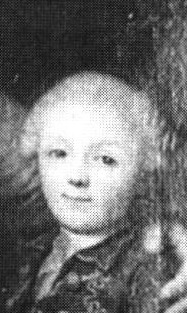
\includegraphics[width=0.88\linewidth,height=0.40\textheight,keepaspectratio]{genealogie/assets/galerie/portraits/portrait-c258023f8640c1103251.jpg}}
\par\vspace{0.10cm}
\galleryworktitle{Double portraits de Antoine Henri I Jordan et son fils Antoine Henri II}
\galleryworkline{Artiste}{Donat Nonotte}
\galleryworkline{Source}{\href{https://books.openedition.org/efr/2016}{Collection privée}}
\end{minipage}
\par\vspace{0.30cm}
\noindent\setlength{\fboxsep}{6pt}\colorbox{GalleryCream}{
\parbox[t]{\dimexpr\linewidth-2\fboxsep-0.4cm\relax}{
\gallerysection{Citations dans l'ouvrage}
{\scriptsize\itshape\color{GalleryMuted} Benoît Coste — Mes souvenirs de soixante ans}\par\vspace{0.10cm}
{\footnotesize\begin{itemize}\setlength{\itemsep}{0pt}\setlength{\topsep}{1pt}\setlength{\parsep}{0pt}\setlength{\parskip}{0pt}
\item Chapitre 2 — p. 16 — \textit{« Mon oncle Jordan fut du nombre de ceux-ci ; heureusement... il fut mis en liberté »}
\end{itemize}}
}
}
\vfill
\noindent\textcolor{GallerySand}{\rule{\textwidth}{0.6pt}}\par
{\scriptsize\color{GalleryMuted}Personnage cité dans les Mémoires de Benoît Coste}\par
\restoregeometry
\endgroup

\clearpage
\thispagestyle{plain}
\begingroup
\newgeometry{top=1.15cm,bottom=1.25cm,left=1.30cm,right=1.30cm}
\raggedbottom

\gallerypageheader
{\LARGE\bfseries\color{GalleryInk} Irénée DE COLOMB}\par
\vspace{0.12cm}
\noindent\textcolor{GallerySand}{\rule{\textwidth}{1.1pt}}\par
\vspace{0.15cm}
{\footnotesize\bfseries\color{GalleryMuted}\MakeUppercase{Relation avec Benoît Coste}}\par
{\large\color{GalleryBordeaux} Le neveu de son épouse Joséphine}\par
\vspace{0.45cm}
\noindent\begin{minipage}[t]{0.52\textwidth}
\noindent\setlength{\fboxsep}{8pt}\colorbox{GalleryCream}{\parbox[t]{\dimexpr\linewidth-2\fboxsep\relax}{\galleryfact{Naissance}{Non renseignée}
\galleryfact{Décès}{Non renseignée}
\galleryfact{Profession}{Non renseignée}}}
\end{minipage}\hfill
\begin{minipage}[t]{0.43\textwidth}\centering
\setlength{\fboxsep}{0pt}\setlength{\fboxrule}{0.8pt}
\fcolorbox{GallerySand}{GalleryCream}{
\parbox[c][0.50\textheight][c]{0.90\linewidth}{\centering
{\fontsize{48}{54}\selectfont\bfseries\color{GalleryBordeaux} ID}\par\medskip
{\small\color{GalleryMuted}Portrait non disponible}\par}}
\end{minipage}
\par\vspace{0.30cm}
\noindent\setlength{\fboxsep}{6pt}\colorbox{GalleryCream}{
\parbox[t]{\dimexpr\linewidth-2\fboxsep-0.4cm\relax}{
\gallerysection{Citations dans l'ouvrage}
{\scriptsize\itshape\color{GalleryMuted} Benoît Coste — Mes souvenirs de soixante ans}\par\vspace{0.10cm}
{\footnotesize\begin{itemize}\setlength{\itemsep}{0pt}\setlength{\topsep}{1pt}\setlength{\parsep}{0pt}\setlength{\parskip}{0pt}
\item Chapitre 28 — p. 232 — \textit{« votre bon oncle Colomb ; il avait un fils âgé de 15 ans, rempli de bonnes qualités ; ce jeune homme, l’espérance de la famille, après une longue et cruelle maladie, succomba »}
\end{itemize}}
}
}
\vfill
\noindent\textcolor{GallerySand}{\rule{\textwidth}{0.6pt}}\par
{\scriptsize\color{GalleryMuted}Personnage cité dans les Mémoires de Benoît Coste}\par
\restoregeometry
\endgroup

\clearpage
\thispagestyle{plain}
\begingroup
\newgeometry{top=1.15cm,bottom=1.25cm,left=1.30cm,right=1.30cm}
\raggedbottom

\gallerypageheader
{\LARGE\bfseries\color{GalleryInk} François \underline{Xavier} NEYRAT}\par
\vspace{0.12cm}
\noindent\textcolor{GallerySand}{\rule{\textwidth}{1.1pt}}\par
\vspace{0.15cm}
{\footnotesize\bfseries\color{GalleryMuted}\MakeUppercase{Relation avec Benoît Coste}}\par
{\large\color{GalleryBordeaux} Le neveu de son épouse Joséphine}\par
\vspace{0.45cm}
\noindent\begin{minipage}[t]{0.52\textwidth}
\noindent\setlength{\fboxsep}{8pt}\colorbox{GalleryCream}{\parbox[t]{\dimexpr\linewidth-2\fboxsep\relax}{\galleryfact{Naissance}{6 mars 1818 — Lyon}
\galleryfact{Décès}{14 novembre 1826 — Lyon}
\galleryfact{Profession}{Non renseignée}}}
\end{minipage}\hfill
\begin{minipage}[t]{0.43\textwidth}\centering
\setlength{\fboxsep}{0pt}\setlength{\fboxrule}{0.8pt}
\fcolorbox{GallerySand}{GalleryCream}{
\parbox[c][0.50\textheight][c]{0.90\linewidth}{\centering
{\fontsize{48}{54}\selectfont\bfseries\color{GalleryBordeaux} XN}\par\medskip
{\small\color{GalleryMuted}Portrait non disponible}\par}}
\end{minipage}
\par\vspace{0.30cm}
\noindent\setlength{\fboxsep}{6pt}\colorbox{GalleryCream}{
\parbox[t]{\dimexpr\linewidth-2\fboxsep-0.4cm\relax}{
\gallerysection{Citations dans l'ouvrage}
{\scriptsize\itshape\color{GalleryMuted} Benoît Coste — Mes souvenirs de soixante ans}\par\vspace{0.10cm}
{\footnotesize\begin{itemize}\setlength{\itemsep}{0pt}\setlength{\topsep}{1pt}\setlength{\parsep}{0pt}\setlength{\parskip}{0pt}
\item Chapitre 28 — p. 227 — \textit{« l’aîné des enfants de ma bonne sœur Mme Neyrat, âgé de moins de dix ans, se trouvait alors très dangereusement malade : Xavier, c’était son nom... enfin les souffrances aiguës qu’endurait ce pauvre petit malade furent terminées par une sainte mort »}
\end{itemize}}
}
}
\vfill
\noindent\textcolor{GallerySand}{\rule{\textwidth}{0.6pt}}\par
{\scriptsize\color{GalleryMuted}Personnage cité dans les Mémoires de Benoît Coste}\par
\restoregeometry
\endgroup

\clearpage
\thispagestyle{plain}
\begingroup
\newgeometry{top=1.15cm,bottom=1.25cm,left=1.30cm,right=1.30cm}
\raggedbottom

\gallerypageheader
{\LARGE\bfseries\color{GalleryInk} Pierre-Adrien NEYRAT}\par
\vspace{0.12cm}
\noindent\textcolor{GallerySand}{\rule{\textwidth}{1.1pt}}\par
\vspace{0.15cm}
{\footnotesize\bfseries\color{GalleryMuted}\MakeUppercase{Relation avec Benoît Coste}}\par
{\large\color{GalleryBordeaux} Le mari de sa belle-sœur Amélie Colomb}\par
\vspace{0.45cm}
\noindent\begin{minipage}[t]{0.52\textwidth}
\noindent\setlength{\fboxsep}{8pt}\colorbox{GalleryCream}{\parbox[t]{\dimexpr\linewidth-2\fboxsep\relax}{\galleryfact{Naissance}{12 janvier 1781 — Lyon}
\galleryfact{Décès}{16 mars 1827 — Caluire-et-Cuire}
\gallerysection{Profession}
\small\begin{itemize}\setlength{\itemsep}{0pt}\setlength{\topsep}{2pt}\setlength{\parsep}{0pt}\setlength{\parskip}{0pt}
\item Écuyer du Roi ; négociant (marchand drapier) ; député.
\end{itemize}}}
\end{minipage}\hfill
\begin{minipage}[t]{0.43\textwidth}\centering
\setlength{\fboxsep}{4pt}\setlength{\fboxrule}{0.8pt}\fcolorbox{GalleryTerracotta}{white}{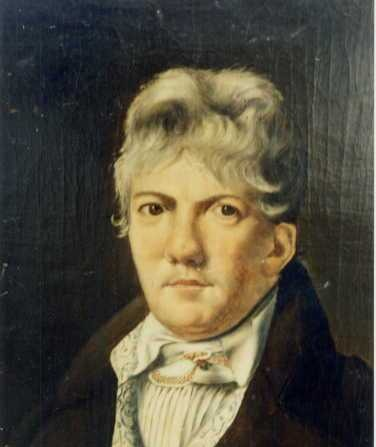
\includegraphics[width=0.88\linewidth,height=0.40\textheight,keepaspectratio]{genealogie/assets/galerie/portraits/portrait-328c338c24cdedd5a61b.jpg}}
\par\vspace{0.10cm}
\galleryworktitle{Portrait de Pierre-Adrien Neyrat}
\galleryworkline{Source}{\href{https://www.geneanet.org/media/public/pierre-adrien-neyrat-543532}{Source en ligne}}
\end{minipage}
\par\vspace{0.30cm}
\noindent\setlength{\fboxsep}{6pt}\colorbox{GalleryCream}{
\parbox[t]{\dimexpr\linewidth-2\fboxsep-0.4cm\relax}{
\gallerysection{Citations dans l'ouvrage}
{\scriptsize\itshape\color{GalleryMuted} Benoît Coste — Mes souvenirs de soixante ans}\par\vspace{0.10cm}
{\footnotesize\begin{itemize}\setlength{\itemsep}{0pt}\setlength{\topsep}{1pt}\setlength{\parsep}{0pt}\setlength{\parskip}{0pt}
\item Chapitre 28 — p. 227 — \textit{« 1827 – Mort d’Adrien Neyrat... Il succomba à une maladie dont il était atteint depuis plus d’un an, laissant à sa veuve si cruellement affligée, trois enfants »}
\end{itemize}}
}
}
\vfill
\noindent\textcolor{GallerySand}{\rule{\textwidth}{0.6pt}}\par
{\scriptsize\color{GalleryMuted}Personnage cité dans les Mémoires de Benoît Coste}\par
\restoregeometry
\endgroup

\endgroup